% VLDB template version of 2020-08-03 enhances the ACM template, version 1.7.0:
% https://www.acm.org/publications/proceedings-template
% The ACM Latex guide provides further information about the ACM template

\documentclass[sigconf, nonacm]{acmart}

\usepackage[a-1b]{pdfx}
\usepackage{amsmath}
\newtheorem{definition}{Definition}
\usepackage{fancyvrb}
\usepackage{bbding}
\usepackage{booktabs}
\usepackage{graphicx}
\usepackage{subcaption}
\usepackage{balance}
\usepackage{hyperref}
\usepackage[inline]{enumitem}
\usepackage[linesnumbered,ruled,noend]{algorithm2e}
\SetKwInOut{Input}{input}\SetKwInOut{Output}{output}
\SetKwProg{Fn}{function}{}{end}
\SetKwSwitch{Match}{Case}{Other}{match}{do}{case}{otherwise}{endcase}

%% The following content must be adapted for the final version
% paper-specific
\newcommand\vldbdoi{XX.XX/XXX.XX}
\newcommand\vldbpages{XXX-XXX}
% issue-specific
\newcommand\vldbvolume{14}
\newcommand\vldbissue{1}
\newcommand\vldbyear{2021}
% should be fine as it is
\newcommand\vldbauthors{\authors}
\newcommand\vldbtitle{\shorttitle}
% leave empty if no availability url should be set
\newcommand\vldbavailabilityurl{http://vldb.org/pvldb/format_vol14.html}
% whether page numbers should be shown or not, use 'plain' for review versions, 'empty' for camera ready
\newcommand\vldbpagestyle{plain}

\begin{document}
\title{SeqStar: A Fast Out-of-Core Property Graph Matching System}

%%
%% The "author" command and its associated commands are used to define the authors and their affiliations.
\author{Yanxuan Cui}
\affiliation{%
  \institution{Tsinghua University}
  \city{Beijng}
  \state{China}
}
\email{cuiyx18@mails.tsinghua.edu.cn}

\author{Kang Chen}
\affiliation{%
  \institution{Tsinghua University}
  \city{Beijng}
  \state{China}
}
\email{chenkang@tsinghua.edu.cn}

\author{Mingxing Zhang}
\affiliation{%
  \institution{Tsinghua University}
  \city{Beijng}
  \state{China}
}
\affiliation{%
  \institution{Sangfor Technologies Inc.}
  \city{Shenzhen}
  \state{China}
}
\email{zhang.mingxing@outlook.com}

\author{Zhiyuan Ma}
\affiliation{%
  \institution{Tsinghua University}
  \city{Beijng}
  \state{China}
}
\email{mazy19@mails.tsinghua.edu.cn}

\author{Juan Yang}
\affiliation{%
  \institution{Beijing HaiZhi XingTu Technology Co., Ltd.}
  \city{Beijng}
  \state{China}
}
\email{yangjuan@stargraph.cn}

\author{Yongwei Wu}
\affiliation{%
  \institution{Tsinghua University}
  \city{Beijng}
  \state{China}
}
\email{wuyw@tsinghua.edu.cn}

\begin{abstract}
  Property graph matching is the most important operation of graph database and has a wide range of applications.
  The problem has been studied extensively, however, on oversimplified graph models.
  Because of the complexity involving directions, multi-edges, labels in property graphs,
  optimizations aimed at simple graphs are not suitable to handle the storage and matching problem of property graphs.
  Moreover, existing approaches rely on huge memory resources to run their system and hinder the popularity of graph technology.

  We present SeqStar, the first out-of-core property graph matching system that can execute real-world complex queries efficiently.
  The storage engine of SeqStar uses a novel \emph{vertex-centric} storage model.
  By storing necessary information together with the vertices,
  SeqStar avoids the random disk access problem of existing work.
  In the graph matching engine, we propose a novel star decomposition algorithm that preserves all the relevant filtering information on stars.
  Therefore, SeqStar can filter out more unnecessary matchings in the very beginning.
  To reduce the memory usage, SeqStar compresses the intermediate results from star matching and performs pipeline join on the compressed data.
  Moreover, we propose a predicate pushdown method for SeqStar to optimize real-world queries.
\end{abstract}


\maketitle

%%% do not modify the following VLDB block %%
%%% VLDB block start %%%
\pagestyle{\vldbpagestyle}
\begingroup\small\noindent\raggedright\textbf{PVLDB Reference Format:}\\
\vldbauthors. \vldbtitle. PVLDB, \vldbvolume(\vldbissue): \vldbpages, \vldbyear.\\
\href{https://doi.org/\vldbdoi}{doi:\vldbdoi}
\endgroup
\begingroup
\renewcommand\thefootnote{}\footnote{\noindent
This work is licensed under the Creative Commons BY-NC-ND 4.0 International License. Visit \url{https://creativecommons.org/licenses/by-nc-nd/4.0/} to view a copy of this license. For any use beyond those covered by this license, obtain permission by emailing \href{mailto:info@vldb.org}{info@vldb.org}. Copyright is held by the owner/author\@(s). Publication rights licensed to the VLDB Endowment. \\
\raggedright{} Proceedings of the VLDB Endowment, Vol. \vldbvolume, No. \vldbissue\ %
ISSN 2150--8097. \\
\href{https://doi.org/\vldbdoi}{doi:\vldbdoi} \\
}\addtocounter{footnote}{-1}\endgroup
%%% VLDB block end %%%

%%% do not modify the following VLDB block %%
%%% VLDB block start %%%
\ifdefempty{\vldbavailabilityurl}{}{
\vspace{.3cm}
\begingroup\small\noindent\raggedright\textbf{PVLDB Artifact Availability:}\\
The source code, data, and/or other artifacts have been made available at \url{\vldbavailabilityurl}.
\endgroup
}
%%% VLDB block end %%%
\section{Introduction}
Graph matching
%~\footnote{There are two kinds of graphs in a graph matching problem: one is the large \emph{data graph}, the other is the much smaller \emph{pattern graph}}
is one of the most important applications of graph databases. In graph matching, a relative small \emph{pattern graph} is used to match subgraphs of a relative large \emph{data graph}.
It is widely used in many fields,
such as Twitter's recommendation systems~\cite{DBLP:journals/pvldb/GuptaSGGZLL14,DBLP:journals/pvldb/SharmaJBLL16},
electronic computer-aided design~\cite{DBLP:conf/dac/OhlrichEGS93},
and protein-protein interaction (PPI) networks~\cite{milenkovic2008uncovering}.
Nowadays, users of industrial graph databases such as Neo4j\footnote{\url{https://neo4j.com}}
can easily model data as property graphs and expressing their queries via the Cypher~\cite{DBLP:conf/sigmod/FrancisGGLLMPRS18} query language.
Although it is convenient to use, the matching process of these industrial graph databases are time and resource consuming.
Many novel subgraph matching algorithms have been proposed~\cite{DBLP:journals/pvldb/SunWWSL12,DBLP:conf/sigmod/HanLL13,DBLP:conf/sigmod/ShaoCCMYX14,DBLP:conf/cloud/SerafiniMS17,DBLP:journals/pvldb/QiaoZC17,DBLP:conf/sigmod/DiasTGM019}, with even orders of magnitude of speedup compared to the industrial graph databases.
However, there are two gaps that hinder these algorithms from being widely adopted in the real-world scenarios:
(1) the gap between the complexity of real-world queries and the simplicity of graphs that the existing algorithms can handle;
(2) the huge memory and high-speed network requirements for the existing algorithms to query on large graphs and the limitation of resource budget.

The property graph is the de facto graph model for real-world graph matching problems.
A property graph is a directed graph with labels attached to vertices and edges.
There may be multiple edges connecting two vertices and even edges for self-loop (edges connecting back to their source vertices).
Moreover, users usually provide extra searching conditions via the WHERE clause~\cite{DBLP:journals/csur/AnglesABHRV17}. However,  current studies mostly deal with simple graph models such as ignoring the directions, labels, or multi-edges. WHERE clause is not considered either~\cite{DBLP:journals/pvldb/SunWWSL12,DBLP:conf/sigmod/HanLL13,DBLP:conf/sigmod/KimLBHLKJ16,DBLP:journals/pvldb/QiaoZC17,DBLP:journals/pvldb/MhedhbiS19}. The optimizations aimed at simple graphs usually heavily rely on the equivalence of vertices~\cite{DBLP:conf/sigmod/HanLL13,DBLP:journals/pvldb/QiaoZC17}, which is harder to find in a property graph because of the complexity of directions and labels. Moreover, in the implementation level, the storage engine designed for simple graph models encounters excessive random disk seeks when matching a real-world property graph.

%This limitation is not only a matter of engineering,
%but also a serious algorithm problem:
%(1) the storage engine designed for simple graph may encounter superfluous random disk reads when matching a property graph;
%(2) the optimizations aimed at simple graph usually rely heavily on the equivalence of vertices~\cite{DBLP:conf/sigmod/HanLL13,DBLP:journals/pvldb/QiaoZC17}, which is harder to find in a property graph because of the complexity of directions and labels.

Existing algorithms rely on main memory for their computation. It is extremely uneconomic for property graph matching problem. The memory needs to hold not only the graph data but also the intermediate results which grow exponentially with respect to the size of graph data. Our experiment shows that a graph with $6.9 \times 10^{7}$ edges could generate $1.7 \times 10^{13}$ rows of matching results.
%(1) The memory needs to hold not only the data graph, but also the intermediate result which grows exponentially with respect to the size of the data graph, as our experiment shows that a graph with $6.9 \times 10^{7}$ edges could generate $1.7 \times 10^{13}$ rows of matching results.
Existing systems~\cite{DBLP:conf/sosp/TeixeiraFSSZA15,DBLP:conf/sigmod/DiasTGM019,DBLP:journals/pvldb/MhedhbiS19} require hundreds of GB of memory to process such graphs. Therefore, we resort to use external memory (such as SSDs) to support property graph matching.
%(2) For distributed approaches, on the one hand it is hard to partition the graph across cluster machines to minimize the communication cost~\cite{DBLP:journals/im/LeskovecLDM09} and have performance problems~\cite{DBLP:conf/sigmod/KimLBHLKJ16},
%one the other hand it is inconvenient and costly for the end user to maintain the cluster nodes~\cite{DBLP:conf/osdi/KyrolaBG12}.

This paper proposes SeqStar, a high performance out-of-core property graph matching system for real-world graphs, which scans the disk sequentially by matching stars (a star contains a root vertex and some leaves which are the neighbors of the root).

%Therefore, in order to match up with the need of real-world problems,a high performance disk-based property graph matching system is desirable.

\subsection*{Contributions}
There are two fundamental components in SeqStar:
the graph storage engine and the graph matching engine. Both are designed specificly to deal with the graph machine problem efficiently.

The storage engine in SeqStar uses the \emph{vertex-centric storage model} which stores the information related to a specific vertex together.
The conventional way to store graphs is the compressed sparse row (CSR) and compressed sparse column (CSC) approach which stores in/out-edges \emph{separately}~\cite{DBLP:conf/sc/PearceGA10,DBLP:conf/osdi/KyrolaBG12}.
CSR is equivalent to storing the graph as adjacency list: the out-edges are stored consecutively on disk.
And CSC stores the in-edges in a similar manner.
In contrast, SeqStar stores the graph data by storing the in/out-edges \emph{together} with the neighbors of each vertex.
With small indexes on disks, pattern matching can quickly get the correct address of relevant data on disk during pattern matching.
We also provide two convenient iterator interfaces to interact with the storage engine.
As a result, SeqStar can avoid random disk seeks and perform graph matching in a sequential disk scan.

For the graph matching engine, SeqStar uses a star decomposition based algorithm to run graph matching.
The analyzer of SeqStar analyzes the graph matching query and select a vertex-cover heuristically as the roots of stars.
%这里加一句如何把原图分解为星型子图
We save all useful filtering information in each star subgraph after decomposition. To reduce the amount of memory that would be used as the storage of intermediate results, a novel compression method, which postponing Cartesian production and digging equivalence classes, is used for star matching results. SeqStar's efficient and scalable pipeline join algorithm is able to process the compressed data. To the best of our knowledge, SeqStar is the first system that integrates the optimization of WHERE clauses in the graph matching algorithm, by pushing the predicates down to the star matching process.

According to our experiments, SeqStar outperforms the state-of-the-art graph querying system Graphflow by up to $26\times$.
And SeqStar can run the queries that Graphflow fails to run due to the out of memory problem.
For complex property graphs that existing academic researches do not support,
we compare SeqStar with industrial graph database Neo4j, and achieved over $2100\times$ speedup.
%To reduce memory usage, we make the following contributions:
%(1) a novel star decomposition algorithm that keeps all the useful filtering information in stars,
%(2) a novel compression algorithm for stars' matching results by postponing Cartesian production and digging equivalence classes,
%(3) an efficient and scalable pipeline join algorithm that is able to process the compressed data directly.

%Moreover, to the best of our knowledge, we are the first one to integrate the optimization of WHERE clauses in the graph matching algorithm, by pushing the predicates down to the star matching process.
%% The conventional graph storage method is the compressed sparse column (CSC) and the compressed sparse row (CSR) format~\cite{DBLP:conf/osdi/KyrolaBG12},
%% which stores the in/out-edges separately for each vertex.
%% However, because of the multi-edges in property graphs, the in/out-edges have to be searched many times to check the matching of a vertex, and result in excessive random disk seeks.
%% To address this challenge, we propose the \emph{vertex-centric storage model} that stores all the necessary information together with the vertices, such that the vertices could be matched in a single sequential scan.

%% Generally speaking, there are two kinds of graph isomorphism algorithm,
%% differing on whether intermediate results are materialized.
%% The first is the backtracking tree-searching method~\cite{DBLP:journals/jacm/Ullmann76,DBLP:journals/pvldb/LeeHKL12,DBLP:conf/sigmod/HanLL13,DBLP:conf/sigmod/KimLBHLKJ16},
%% which does not generate intermediate results but have scaling problems~\cite{DBLP:conf/cloud/SerafiniMS17}.
%% The second is the join-based algorithm~\cite{DBLP:journals/pvldb/LaiQLC15,DBLP:journals/pvldb/QiaoZC17,DBLP:journals/pvldb/SunWWSL12,DBLP:journals/pvldb/MhedhbiS19},
%% which decomposes the pattern graph into smaller matching unit and materialize the intermediate results,
%% and the final result is obtained by joining on these intermediate results.
%% Because of the notorious poor locality of graphs,
%% enormous amount of random disk accesses would be encountered for an out-of-core tree-searching approach.
%% Based on this observation, this paper designs a join-based property graph matching algorithm.

%% The most fundamental problem of a graph matching algorithm is to determine the basic matching unit.
%% Edges are the simplest matching units, however, intermediate results much larger than the data graph would be generated and result in costly join operations.
%% To avoid excessive joins, authors use more complex structures i.e.,
%% frequent subgraphs, multi-hop edges, or cliques as their matching unit~\cite{DBLP:conf/sigmod/HeS08,DBLP:conf/edbt/ZhangLY09,DBLP:journals/pvldb/QiaoZC17}, however,
%% these algorithms rely on super-linear indices~\cite{DBLP:journals/pvldb/SunWWSL12}.
%% To address this challenge, we make a balance by choosing stars as our basic unit.
%% And our star decomposition algorithm is enhanced such that the stars keep as much filtering information as possible.
%% Our experiment shows that this enhancement could reduce the intermediate results by up to $43\%$ of the existing works.

%% However, the stars' matching results could still be very large because the matching results grow exponentially with respect to the data graph,
%% e.g., a 129M graph could easily eat up hundreds or even thousands GB of memory to store the intermediate results.
%% Inspired by VCBC~\cite{DBLP:journals/pvldb/QiaoZC17}, we develop a novel compression algorithm for star' matching result by postponing the costly Cartesian product and digging the equivalence classes in the leaves of the star.
%% The compression ratio is quite impressive, as high as $10^8$,
%% and we find that the size of the compressed star's matching results takes less than $23\%$ the space to store the graph,
%% which can even fit into the main memory of a laptop.

\section{Background}\label{sec:background}
This section introduces the formal definition of property graphs, and then discusses the property graph matching problem.
\subsection{Property Graph Model}
A \emph{property graph} is a directed vertex-labeled edge-labeled multigraph with self-edges,
and key-value properties are stored on vertices and edges.
We now provide the formal definition of a property graph.
\begin{definition}[Property Graph~\cite{DBLP:journals/csur/AnglesABHRV17}]
  A property graph $G$ is a tuple $(V, E, \rho, \lambda, \sigma)$, where:
  \begin{enumerate}[noitemsep,label={(\arabic*)}]
  \item $V$ is a finite set of vertices.
  \item $E$ is a finite set of edges such that $V$ and $E$ have no elements in common.
  \item $\rho: E \rightarrow (V \times V)$ is a total function.
    Intuitively, $\rho(e) = (v_1, v_2)$ indicates that $e$ is a directed edge from $v_1$ to $v_2$.
  \item $\lambda :(V \cup E) \rightarrow L$ is a total function where $L$ is a set of labels.
    Intuitively, if $v \in V, \rho(v) = l$ (respectively, $e \in E, \rho(e) = l$),
    then $l$ is the label of vertex $v$ (respectively, edge $e$).
  \item $\sigma: (V \cup E) \times Prop \rightarrow Val$ is a partial function with $Prop$ a finite set of properties and $Val$ a set of values.
    Intuitively, if $v \in V, p \in Prop, \sigma(v, p) = s$ (respectively, $e \in E, p \in Prop, \sigma(e, p) = s$),
    then $s$ is the value of property $p$ for vertex $v$ (respectively, edge $e$) in the property graph $G$.
  \end{enumerate}
\end{definition}
For simplicity, in this paper, we do not discuss the properties i.e., $\sigma$ in $G$,
because similar techniques can be used as processing the labels $\lambda$.
Thus, the property graph $G$ can be denoted by $(V(G), E(G), \rho_G, \lambda_G)$.
Please note that the total function $\rho_G$ is necessary, in general,
we cannot identify an edge simply by the starting and ending vertices such as $(u_1, u_2)$ as can be done in the simple graph model,
because multiple edges may appear between the two vertices.
However, we may use the $(u_1, u_2)$ notation if all we care about is that there exist at least one edge between $u_1$ and $u_2$.
\begin{definition}[Vertex Cover]
  A vertex cover $V_c$ of a property graph $G$ is a subset of $V(G)$ such that
  $\forall e \in E(G), \rho_G(e) = (u, v) \implies u \in V_C \lor v \in V_C$.
\end{definition}
\subsection{Property Graph Matching Problem}
\begin{definition}[Subgraph]
  A property graph $F$ is called a subgraph of a property graph $G$, written $F \subseteq G$, if
  $V(F) \subseteq V(G)$, $E(F) \subseteq E(G)$, $\rho_F$ is a restriction of $\rho_G$, and $\lambda_F$ is a restriction of $\lambda_G$.
\end{definition}
Let $G$ be any property graph, and let $S \subseteq V(G)$, then the \emph{induced subgraph} $G[S]$ is the graph whose vertex set is $S$ and whose edge set consists of all of the edges in $E(G)$ that have both endpoints in $S$.
\begin{definition}[Property Graph Isomorphism]
  Two property graphs $G$ and $H$ are isomorphic, written $G \cong H$,
  if there exists bijections $\theta: V(G) \rightarrow V(H)$ and $\phi: E(G) \rightarrow E(H)$ such that
  $\rho_G(e) = (u, v)$ if and only if $\rho_H(\phi(e)) = (\theta(u), \theta(v))$,
  $\lambda_G(v) = \lambda_H(\theta(v))$ for all $v \in V(G)$
  and $\lambda_G(e) = \lambda_H(\phi(e))$ for all $e \in E(G)$;
  Such a pair of mappings is called an isomorphism between $G$ and $H$.
\end{definition}
The bijection $\theta: V(G) \rightarrow V(H)$ is the key in the definition of property graph isomorphism,
because the bijection $\phi: E(G) \rightarrow E(H)$ is straightforward if $\theta$ is fixed.
However, due to automorphism, where an \emph{automorphism} of a graph is an isomorphism of the graph to itself,
the bijection $\theta$ may not be unique.
\begin{definition}[Property Graph Matching]\label{def:property_graph_matching}
  Given a data property graph $D$, a pattern property graph $P$ and a searching condition $\psi: PG \rightarrow B$ with $PG$ the set of property graph and $B$ the set of Boolean values,
  the property graph matching problem is to report the set $\mathcal{I} = \{F | F \subseteq D, F \cong P, \psi(F) = true\}$.
\end{definition}
Authors of previous works usually omit the searching condition $\psi$ in their definition of graph matching~\cite{DBLP:conf/sigmod/ShaoCCMYX14,DBLP:journals/pvldb/LaiQLC15,DBLP:conf/sigmod/KimLBHLKJ16,DBLP:journals/pvldb/QiaoZC17}.
And they adopt a loosely related technique called \emph{symmetry-breaking}~\cite{DBLP:conf/recomb/GrochowK07},
which ensures there is a unique bijection $\theta: V(P) \rightarrow V(F)$ by providing a partial order on $V(P)$ after exploiting the automorphism of $P$.
However, as we have stated before, the WHERE clause is a ubiquitous part of the query language of a graph database.
Users of a real-world graph database usually provide their self-defined searching condition $\psi$ to filter out unnecessary matchings not only symmetry-breaking conditions.
Thus, the searching condition we defined here can be viewed as a super set of symmetry-breaking.
We add the searching condition in the definition because it is actually a part of the property graph matching problem,
and we also found that it can be decomposed and pushed down to lower phase to boost the evaluation of graph matching (Section~\ref{sec:framework}).

A property graph is always directed.
However, in some cases such as friendship, there is no need to pay attention to the directions of the edges.
In order to support this kind of relationship, a naive approach is to add a duplicate edge in opposite direction for each edge in the data graph.
More elegantly, we allow the pattern graph $P$ to contain undirected edges.
Users can simply ignore the direction by providing undirected edges in $P$ like in industrial graph databases such as Neo4j.

\section{Overview of SeqStar}\label{sec:framework}
We demonstrate the workflow of SeqStar in this section,
and use an example to show the query processing stages.
\subsection{SeqStar Workflow}
\begin{figure}[ht]
  \centering
  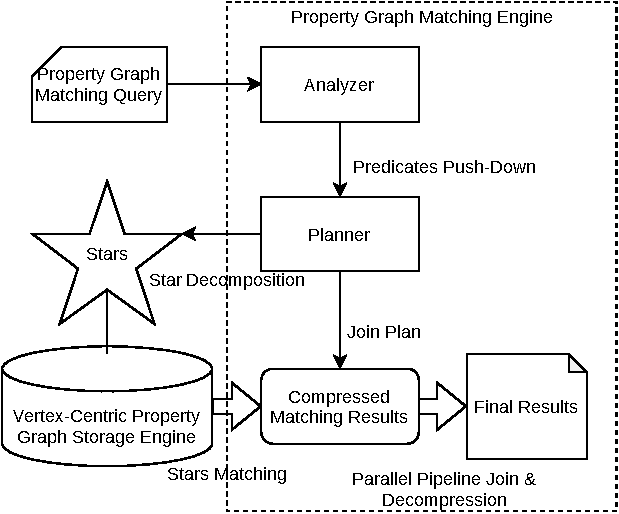
\includegraphics[width=0.48\textwidth]{img/architecture.pdf}
  \caption{SeqStar workflow.}\label{img:architecture}
\end{figure}
Figure~\ref{img:architecture} shows the workflow of SeqStar. There are mainly two building blocks in SeqStar: the storage engine and the property graph matching engine.
Both are specially designed to deal with the property graph matching problem efficiently.

Traditional graph storage engines such as used in graph databases store the in-edges and out-edges separately for each vertex.
Because of the complexity in property graphs,
such a storage method is not suitable and would incur many unnecessary random disk accesses.
We develop a vertex-centric property storage model to store all information related to one vertex together to address the problem (\S\ref{sec:storage}).


Based on the storage model,
we propose an efficient property graph matching engine that is able to execute real-world complex queries (\S\ref{sec:match}).
The core of the graph matching engine is the planner, which  decomposes the pattern into a series of stars.
Compared with existing works, we take a step further by introducing
(1) a matching result compression algorithm which reduces the cost of materializing intermediate results,
(2) a predicate pushdown optimizer that is able to filter out unnecessary matchings in early stages and mitigate the burden of the join process.
\subsection{Query Processing Stages}
Here is an example of how a concrete query gets executed in SeqStar.
Consider the Cypher (Neo4j's graph query language) query in Figure~\ref{img:cypher_query},
which generates the pattern graph in Figure~\ref{img:running_example} (b):

\begin{figure}[ht]
  \begin{Verbatim}[fontsize=\small]
    MATCH (u1:Person)-[:FOLLOWS]->(u2:Person)-[:FOLLOWS]->(u1),
          (u1)-[:FOLLOWS]->(u3:Person)-[:FOLLOWS]->(u1),
          (u1)-[:REPOSTS]->(u4:Media),
          (u2)-[:LIKES]->(u4)<-[:LIKES]-(u3)
    WHERE u2 > u1 AND NOT (u3 <= u1 OR u4 >= 8)
  \end{Verbatim}
  \caption{Example query.}\label{img:cypher_query}
\end{figure}

\begin{figure*}[ht]
  \centering
  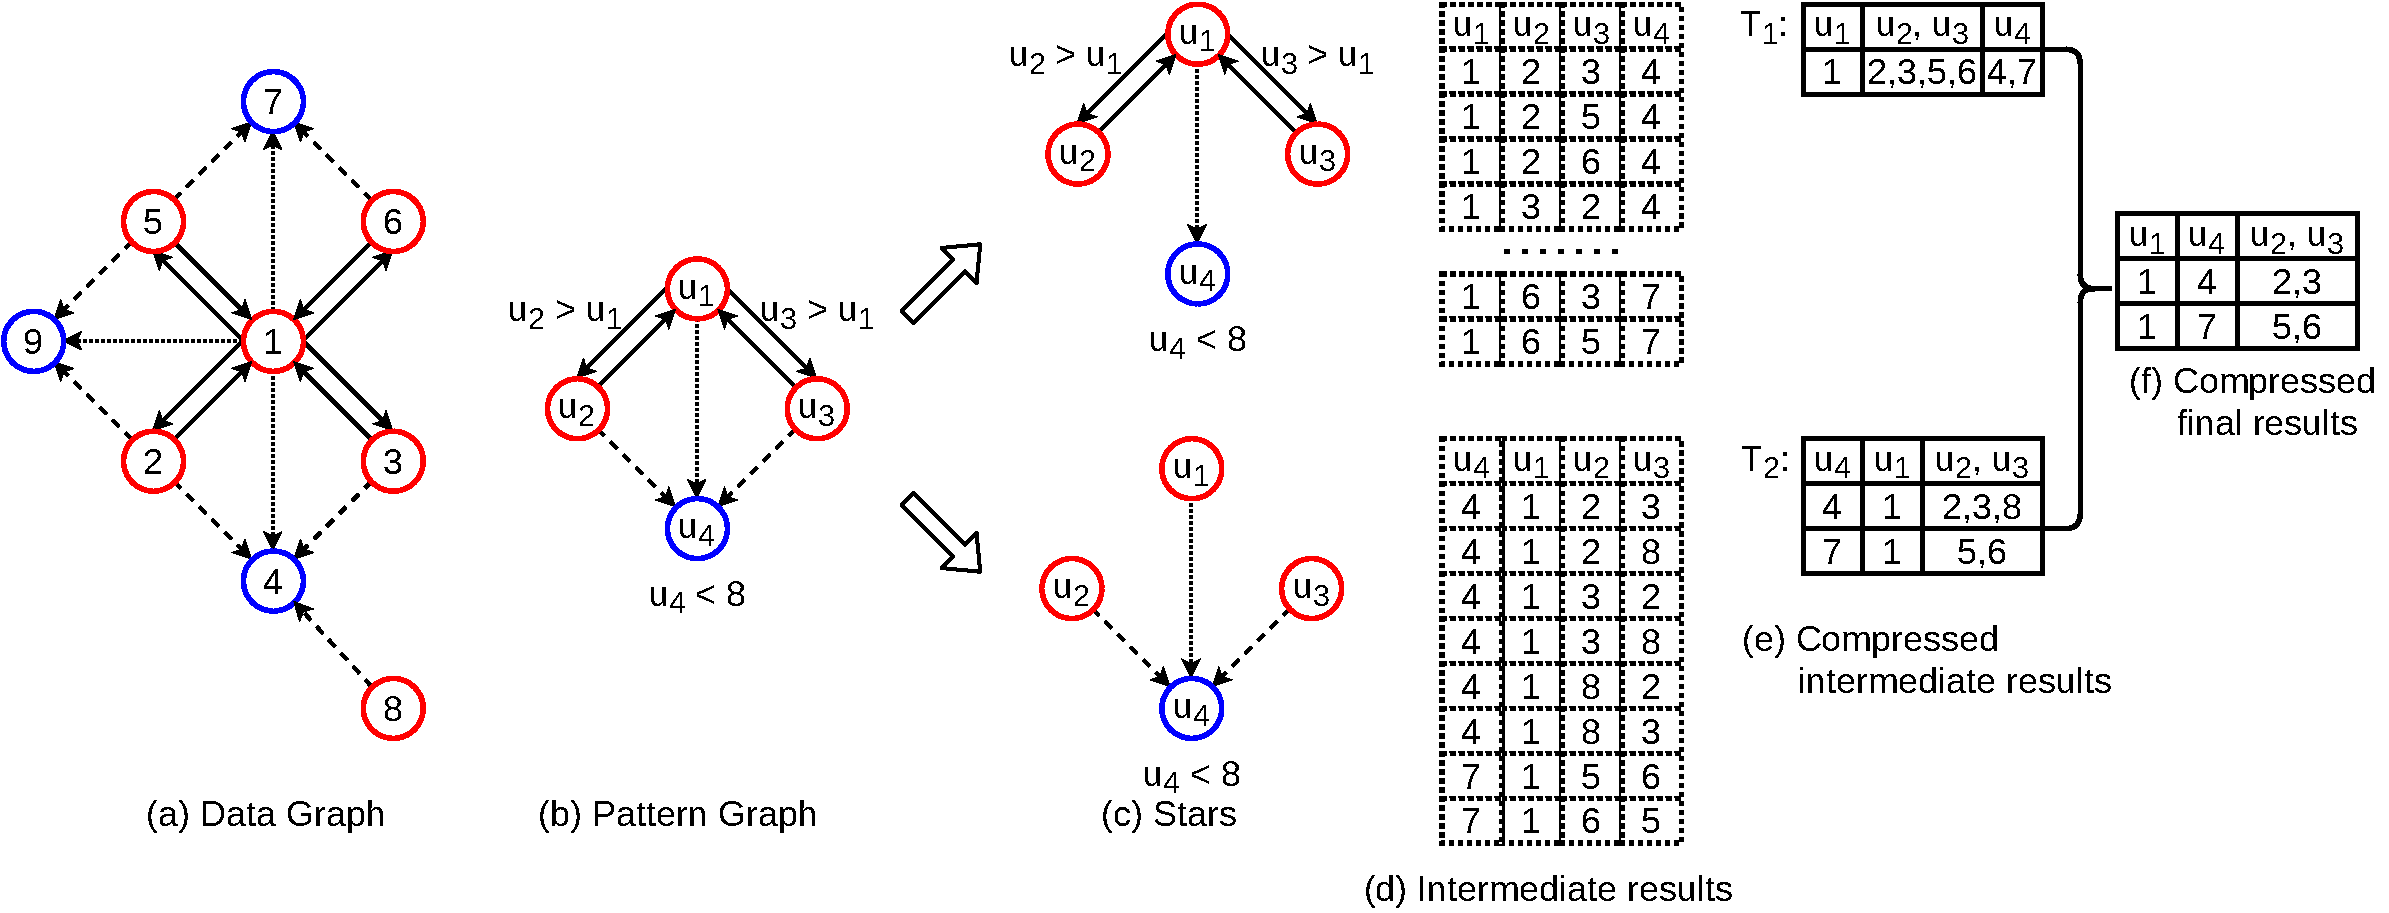
\includegraphics[width=\textwidth]{img/running_example.pdf}
  \caption{Working stages of the example query.}\label{img:running_example}
\end{figure*}

The analyzer firstly analyzes the WHERE clause and extract useful filtering information for early stage filtering.
SeqStar rewrites the WHERE clause to AND-separated expressions `$u_2 > u_1$ AND $u_3 > u_1$ AND $u_4 < 8$' by applying De Morgan's law.
The searching conditions $u_2> u_1$, $u_3 > u_1$ and $u_4 < 8$ are then attached to the pattern graph (Figure~\ref{img:running_example} (b)).
Based on the analysis result and the statistical information of the data graph,
the planner dynamiclly selects a connected vertex cover ($u_1, u_4$) in the pattern as the roots of stars.
The star generating algorithm keeps all the relevant edges and additional searching conditions in order to filter out unnecessary matchings as early as possible.

With the help of SeqStar's vertex-centric storage engine,
all the stars can be matched by only one sequential scan on the data graph (\S\ref{sec:match_star}).
For example, to match star $S_2$,
SeqStar seeks to the vertices labeled with ``Media'' (colored in blue) quickly by searching the index in the storage engine.
The candidate vertices $4, 7, 9, 10$ (vertices are identified by their IDs in integers) may match the root $u_4$.
Then SeqStar scans the candidate vertices sequentially and finds that only vertex $4, 7$ can be matched (vertex $9$ and $10$ violate the constraint $u_4 < 8$).

The intermediate results from star matching are not stored as conventional flat and incarnated rows. Instead, SeqStar compresses the intermediate results and uses pipeline joins without incarnation of some intermediate rows.

SeqStar compresses the intermediate results by digging equivalence classes among vertices and postponing Cartesian product to reduce memory usage (\S\ref{sec:match_compress}).
In the decomposed stars, $u_2$ and $u_3$ have the same label, and they also have the same connections to the root $u_1$ or $u_4$ ($u_2 > u_1$ and $u_3 > u_1$ are equivalent in this case because they both represent the filter $f(x): x > u_1$).
We say that $u_2$ and $u_3$ both belong to the same \emph{neighbor equivalence class}.
For each neighbor equivalence class, the matched vertices are stored together as an \emph{image set}.
For example $\{2, 3, 5, 6\}$ in $T_1$ is the image set of $u_2$ and $u_3$.
An \emph{image set} is the basic structure to hold the intermediate results.
While scanning each vertex $v$ in the data graph,
SeqStar checks the neighbors of $v$ and stores the matched neighbors together as image sets.
To match the star $S_2$,
for each candidate e.g., vertex $4$, SeqStar scans the neighbors of vertex $4$ and finds that $u_1$'s image set is $\{1\}$,
the image set of $u_2, u_3$ is $\{2, 3, 8\}$.
The tuple $(4, \{1\}, \{2, 3, 8\})$ is then appended to the compressed intermediate results, as a \emph{SuperRow}.
Note that the first column contains only one vertex, which matches the root of a star.

Finally, SeqStar performs the joins on SuperRows to obtain the final results (\S\ref{sec:match_join}) without the incarnation of intermediate rows. The planner generates a join order ($T_1 \Join T_2$ in this case) based on the statistical information of the SuperRows.
For each SuperRow $R_1$ in $T_1$, SeqStar scans the image set of $u_4$ and finds the corresponding SuperRow $R_2$ in $T_2$.
The join result of $u_2$, $u_3$ is obtained by the intersection if the corresponding columns of $R_1$ and $R_2$,
i.e., $\{2, 3, 5, 6\} \cap \{2, 3, 8\} = \{2, 3\}$, $\{2, 3, 5, 6\} \cap \{5, 6\} = \{5, 6\}$.
If more than two stars are decomposed from the pattern graph,
instead of join them one by one,
the planner in SeqStar will generate a pipeline plan to multi-join on the SuperRows.
By doing so, no new intermediate rows will be generated.
SeqStar generates the compressed final results in a stream manner.
The decompression by Cartesian product to get the final results is not performed     unless required. The compression and pipeline joining can efficiently reduce the memory consumption during computation.

%and the decompression is done by doing Cartesian production on the fly to report the final answer.

%% The vertex-centric storage engine is designed to be I/O efficient and support the real-world property graph well.
%% The conventional way to store graphs on disk is to store the in/out-edges separately for each vertex,
%% via the compressed sparse column (CSC) and the compressed sparse row (CSR) format~\cite{DBLP:conf/sc/PearceGA10}.
%% However, we find that the conventional graph storing method has limitations for real-world property graph:
%% because of the existence of multi-edges,
%% one has to scan all the in/out-edges to check whether a vertex could be matched if the graph is stored in the traditional way, which is time consuming and I/O inefficient.
%% To address this problem, in Section~\ref{sec:storage},
%% we propose a vertex-centric storage model by storing all the necessary local information together with the neighbors,
%% such that all the unnecessary scanning are avoided.
%% Moreover, we develop two kind of simple indices to boost the searching of vertices, which reduces I/Os even further.

%% The property graph matching engine adopts a join-based method.
%% Generally speaking, there are two kinds of approaches to solve the graph isomorphism problem:
%% one is the tree-based searching algorithm~\cite{DBLP:journals/jacm/Ullmann76,DBLP:conf/sigmod/HanLL13}, and the other is the join-based method~\cite{DBLP:journals/pvldb/LaiQLC15,DBLP:journals/pvldb/QiaoZC17,DBLP:journals/pvldb/MhedhbiS19}.
%% Because of the poor locality of graphs, significant random disk reads may incur when implementing an out-of-core tree-based searching algorithm~\cite{DBLP:conf/sigmod/KimLBHLKJ16}, and thus we choose the join-based approach.
%% The most fundamental problem for a join-based algorithm is to choose the basic matching unit.
%% A straightforward approach is to match the edges of a pattern and then join on the edges' matching results,
%% however, incredible amount of useless intermediate results would be generated by doing so,
%% because an edge contains very little filtering information such as degrees and neighborhood structures.
%% Some authors address the problem by joining on more complex structures such as multi-hop edges or frequent subgraphs,
%% however, it is costly to pre-build proper indices and they require super-linear space~\cite{DBLP:journals/pvldb/SunWWSL12}.
%% Based on these observation, we make a trade-off by choosing stars as our basic unit.
%% Thanks to our vertex-centric storage model, in Section~\ref{sec:match_star}, we'll show that we could scan the huge data graph at most once to obtain the stars' matching results, and all the disk accesses are sequential.
%% Some authors also use star-like structures as their join unit~\cite{DBLP:journals/pvldb/SunWWSL12,DBLP:journals/pvldb/LaiQLC15}, however, we take more steps further by improving the star decomposition algorithm to contain as much filtering information as possible, and our experiment shows that our algorithm could reduce the size of intermediate to $???\%$ and obtain $???\times$ speed-up.

%% For real-world billion node graphs, the intermediate result is another challenge that must be conquered.
%% Even though we could use stars to filter out many unnecessary matchings,
%% the intermediate results could still be gigantic for really huge graphs.
%% Moreover, the intermediate result grows exponentially with respect to the size of the data graph,
%% and they could be even larger than the original data graph.
%% Our experiment shows than a data graph with $???x$ edges may generate $???x$ ($???\times$) rows of matching results.
%% Most of the existing work rely on large physical memory to store the huge intermediate results,
%% which is financially expensive and limit the application of property graph matching.
%% To solve the challenge, in Section~\ref{sec:match_compress}, we design a very compact compression algorithm for stars' matching results.
%% By postponing the Cartesian product and digging the equivalence classes among the vertices in a star,
%% the compression ratio reaches as high as $10^{11}$ (Section~\ref{sec:experiments}).
%% And the compressed data is designed to be written sequentially such that we could write them to disk efficiently when memory is limited, i.e., solving a large property graph matching problem on a laptop.
%% Moreover, in Section~\ref{sec:match_join}, we propose a parallel pipeline join algorithm that is able to join directly on the compressed data.

%% A graph matching query consists two parts: the pattern graph description part (the MATCH clause) and the constraint specification part (the WHERE clause).
%% For example, Figure~\ref{img:cypher_query} shows the Cypher query (Neo4j's graph query language) corresponds to the pattern in Figure~\ref{img:pattern_graph}.
%% Existing graph matching frameworks usually neglect the WHERE clause,
%% because they could always be applied as filters after the graph isomorphism result is obtained.
%% However, the WHERE clause is ubiquitous in real-world property matching queries and they contains many user specified constraints~\cite{DBLP:journals/csur/AnglesABHRV17},
%% it is desirable to push them down to the graph isomorphism searching phase and make full use of these searching constraints.
%% However, it is still challenging to pushdown the predicates, because it depends on the graph matching algorithm and the predicates may involve in vertices among different stars.
%% To address this problem, in Section~\ref{sec:match_optimize}, we propose a novel predicates splitting algorithm that is able to extract useful searching constraints from the WHERE clause and push them down to the star matching process,
%% and reduces the intermediate results further.
%% Our experiment shows that, we could save $???\%$ of the space if the WHERE clause is handled properly,
%% and the overall performance is $???\times$ better then the naive approach.

\section{Vertex-Centric Storage for Property Graph}\label{sec:storage}
%The random access problem is a well known hard problem for out-of-core systems, especially for the graph related problem, which is notorious for its poor locality~\cite{DBLP:conf/osdi/KyrolaBG12}.

Many graph computing frameworks store graphs on disk using the double list method:
storing the in-edges and out-edges \textbf{separately} for each vertex,
via the compressed sparse column (CSC) and the compressed sparse row (CSR) format~\cite{DBLP:conf/sc/PearceGA10}.
However, this separation incurs excessive random access on real-world property graph because we need to get the information for in/out edges during pattern matching.

Instead, SeqStar stores the graph data in a vertex-centric way which stores all the information related to one vertex \textbf{together}.
With small indexes on disks, pattern matching can quickly get the correct address of relevant data on disk during pattern matching. Because all the related information is stored together, SeqStar can make sure that all disk reads are sequential.

Moreover, by using the property graph matching engine that will be discussed in the next section,
the huge data graph will be read at most once.
\subsection{Scan the Data Graph Sequentially}
%The property graph matching problem requires the complete connection information between vertices,
%however, the conventional double list storage method break up the completeness and results in random disk accesses.

Consider the example in Figure~\ref{img:running_example}.
If two vertices in the data graph, say $v_i$ and $v_j$, are supposed to match $u_1$ and $u_2$,
we must be sure that $v_i$ and $v_j$ follows each other at the same time.
This kind of neighbor checking is the most essentially building block of a property graph matching engine.

In the data graph, vertex $1$ has $4$ in-edges and $7$ out-edges.
Suppose that they are stored separately in the traditional way.
In order to determine whether vertex $1$ could match $u_1$,
one has to scan the in-edges (or equally, the out-edges) of vertex $1$ and then check whether the visited neighbor is in the out-edges (or in-edges) list.
Such a scan and check method would significantly slow down the graph matching process,
because the checking process results in random disk reads.
For real world power-law graphs, where the celebrities or trending topics have a huge amount of followers, this phenomenon greatly exacerbate the random access problem.
%the in/out-edges lists stored on disk have to be swapped in and out frequently during the scan and check process as a result of the random disk access pattern.
%% Multiple edges between $u_1$ and $u_2$ make things even worse.
%And it would be more complicated if there are more than two edges between $u_1$ and $u_2$ in the pattern graph.

On the contrarily, SeqStor's vertex-centric storage keeps the necessary connection information together for graph matching.
Figure~\ref{img:data_example} shows the logical structure for the data graph in Figure~\ref{img:running_example}.
The specific edge information (direction, types) could be obtained by the stored edge labels, i.e., the top labels associate to the out-edges and the bottom labels associate to the in-edges (Figure~\ref{img:data_example}).

\begin{figure}[ht]
  \centering
  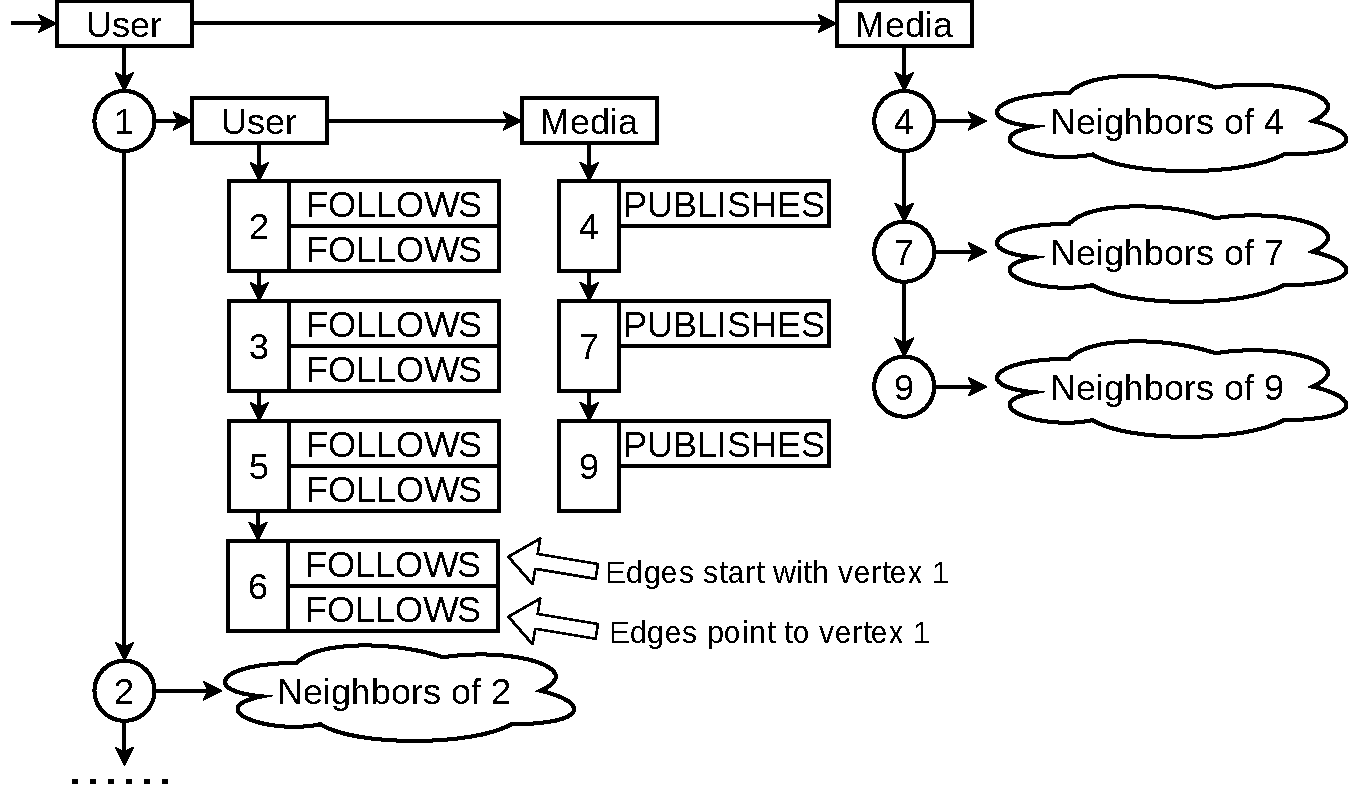
\includegraphics[width=0.5\textwidth]{img/data_example.pdf}
  \caption{Vertex-centric graph data storage.}\label{img:data_example}
\end{figure}

By using the vertex centric graph data storage, the neighborhood checking process can be accomplished efficiently within a sequential disk scan.
For $S_1$ in Figure~\ref{img:running_example},
to check the neighbors of vertex $1$, SeqStar scans the neighbors $2, 3, 5, 6$ and $4, 7, 9$ sequentially.
No random disk access appears during the whole process.
\subsection{Graph Data Indexes}
%Despite of the fact that the size of the whole data graph could be gigantic,we may only care a fraction of the graph by specify the labels in our query for a concrete graph matching problem.
There are two basic operations in a graph matching engine:
(1) Given a data vertex, retrieve its neighbors with a specific label;
(2) Given a vertex label, retrieve the vertices with the label.
%% In the following paragraphs, we'll show how to make the two operations efficiently by adding a few simple but efficient indices to the vertex-centric storage engine,
%% which reduces the searching space and I/O significantly.

Consider the data graph in Figure~\ref{img:running_example}.
One may want to study only the relationships among users.
For vertex $1$ in the figure,
no matter how much social media she has published or viewed we could just ignore all of them in this specific problem.
%% A straightforward idea is to group the neighbor vertices with the same label together when storing the vertices.
%% However, if the neighbor vertices were stored in the traditional in/out-edge double lists method,
%% we have to group them twice and then still face the information insufficient problem as we discussed in the previous subsection.
%% As for our vertex-centric storage method,
For SeqStor's vertex-centric storage method,
the index could be added to the storage engine easily as shown in Figure~\ref{img:data_example}.
These indexes are key-value pairs mapping the vertex labels to the starting/ending position of the neighbors on disk.
Since it is used to locate only the neighbors of a specific vertex, we refer to this kind of index as \emph{local index}.
With the help of local index, we could skip all the useless neighbor vertices and only scan the necessary ones.
%% \begin{figure}[ht]
%%   \centering
%%   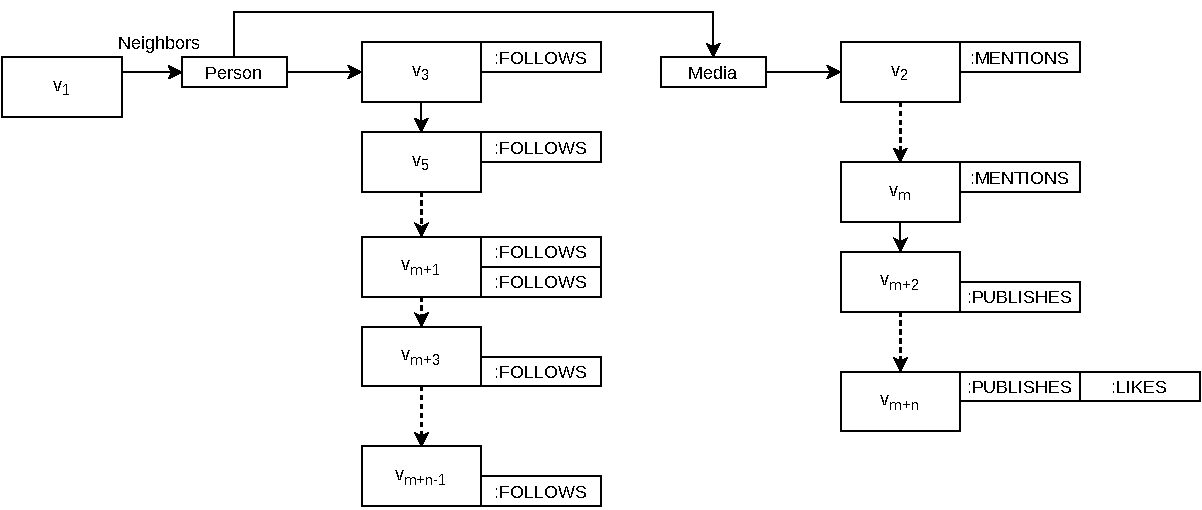
\includegraphics[width=0.48\textwidth]{img/data_neighbors.pdf}
%%   \caption{The vertex-centric storage structure of the celebrity $v_1$ in Figure~\ref{img:celebrity_star}.}\label{img:data_neighbors}
%% \end{figure}

From a higher perspective, in order to solve a property graph matching problem,
one need to firstly select a root vertex in the data graph.
%% regardless of the concrete graph matching algorithm whether it is tree based or join based.
There is no need to scan all the vertices in a billion node data graph if we only care about vertices with the specific labels.
Just like the local index we discussed above, we could add a global index which contains key-value pairs that maps the labels to the corresponding position on disk (Figure~\ref{img:data_example}).

The super-linear index problem of existing work was pointed out by~\cite{DBLP:journals/pvldb/SunWWSL12},
where indexes grow \emph{super-linearly} with respect to the \emph{edges}.
In contrast, indexes of SeqStar grows \emph{linearly} with respect to the \emph{vertices}.
In SeqStar, the length of global index is the length of vertex labels ($l$),
and the size of local indexes is bound to $l \times n$ ($n$ is the length of vertices).
%% In summery, for a property graph matching problem, we could quickly jump to the domain of interest with the help of the global index, and then scan and check only the necessary neighbors with the help of our local index.
%% After jump to the correct position, all the disk reads are sequential.
%% \begin{figure}[ht]
%%   \centering
%%   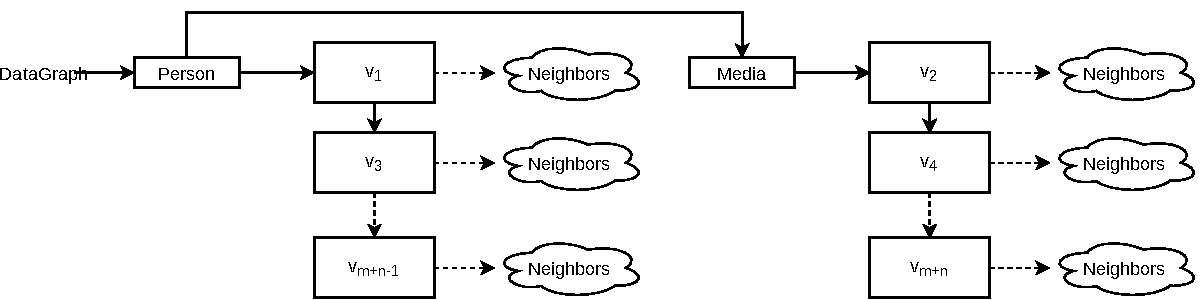
\includegraphics[width=0.48\textwidth]{img/data_vertices.pdf}
%%   \caption{The storage structure overview of the data graph in Figure~\ref{img:celebrity_star}.}\label{img:data_vertices}
%% \end{figure}
\subsection{Remarks on the Implementation of the Storage Method}\label{sec:storage_iterators}
For applications that need to perform the two basic operations (visiting vertices and visiting the neighbors),
we define two iterators as the interface to visit the data graph:
\begin{enumerate}[noitemsep]
\item \textsc{VertexIter}: Given a vertex label, it iterates through the vertices with the specified label ordered by the ID of vertices;
\item \textsc{NeighborIter}: Given a data vertex and a label, it visits the neighbors with the label, the neighbors are also sorted by the IDs.
\end{enumerate}
%% In Section~\ref{sec:match} we'll show that the sorting constraint could boost the matching of property graphs.

These iterators could be implemented efficiently by using SeqStar's vertex-centric storage model.
And we also provide a compact disk format implementing the vertex-centric storage model in Figure~\ref{img:data_graph}.
Vertices are sorted by their IDs, and we store in/out-degrees as early filters when scanning the vertices.
Edge labels are stored as integers here, however, bitmap could also be used for higher performance.
The \textsc{VertexIter} just searches the global index and then visits the disk data sequentially;
The \textsc{NeighborIter} scans the neighbors with the help of the local index.

Note that the vertex-centric storage model is not restricted to this disk format.
In fact, as long as a storage engine could implement the two iterators efficiently,
it could implement the vertex-centric storage model well.
For example, the sorted vertices could be replaced with B-tree to make the insertion/deletion operation easier for dynamic graphs.
%% It is also possible to implement the vertex-centric storage model in memory as buffer cache for existing graph databases to achieve better locality.
Moreover, we are now working on implementing the vertex-centric storage model on top of relational database to embrace the power of the half-century-year-old mature technology.
\begin{figure}[ht]
  \centering
  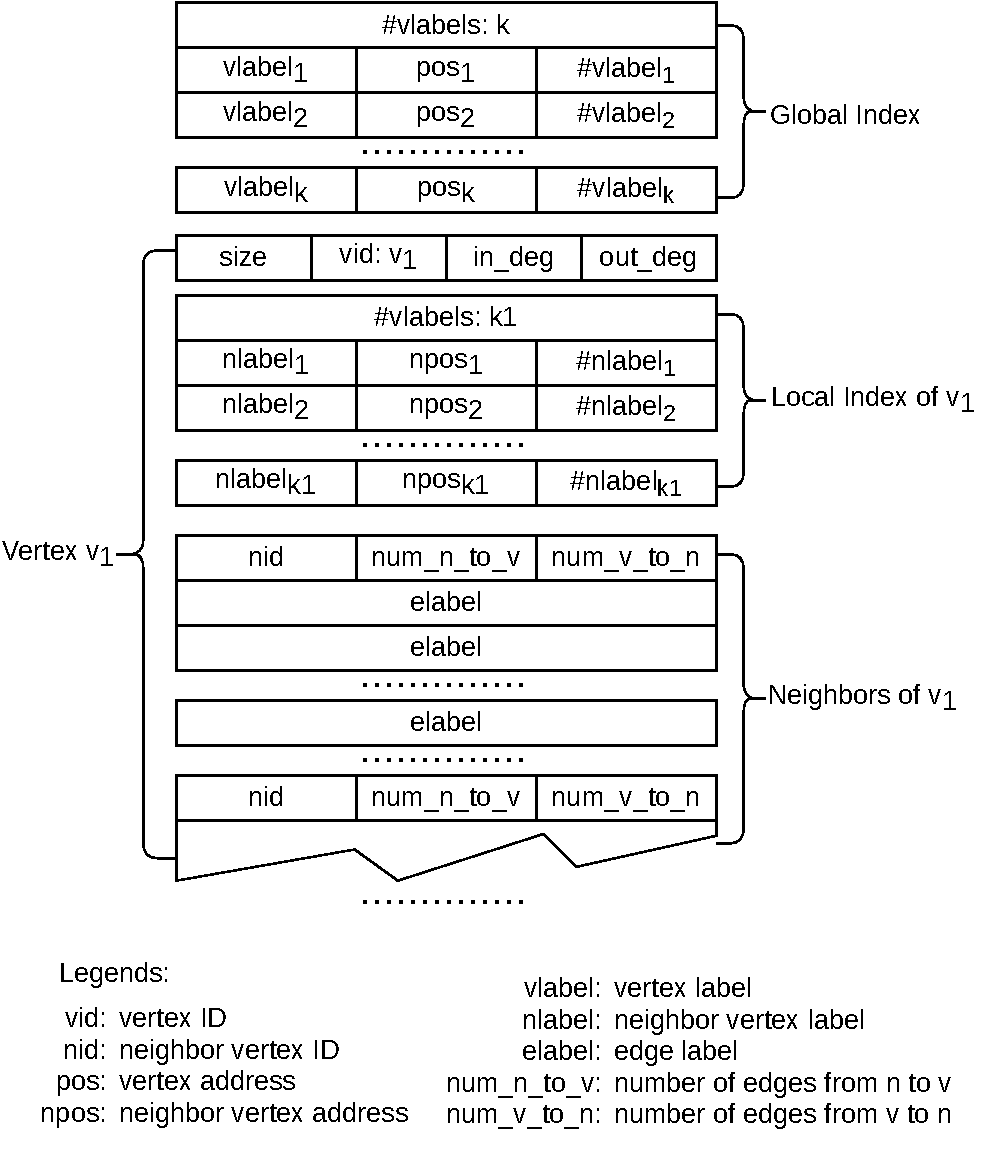
\includegraphics[width=0.48\textwidth]{img/data_graph.pdf}
  \caption{An I/O efficient property graph storage method that can boost the graph matching process.}\label{img:data_graph}
\end{figure}

\section{Property Graph Matching Engine}\label{sec:match}
%% Real world billion-node property graph can easily eat up hundreds of gigabytes,
%% apart from that, even more spaces are required to store the intermediate results,
%% which makes it financially impossible to solve the realistic property graph matching problem totally in memory.
%% However, challenges have to be faced when developing an out-of-core property graph matching engine,
%% because of the infamous random disk access problem.

%In this section, we present the property graph match engine of SeqStar.
%Based on the vertex-centric storage engine, SeqStar avoids random disk accesses when scanning the graph data file.

SeqStar's graph matching engine is based on the vertex-centric storage to avoid the random disk seeks.
The intermediate results explosion problem is resolved by adopting a compression algorithm which based on equivalence classes to postpone Cartesian product.
Moreover, an efficient pipeline join method can work on compressed data directly.
\subsection{Star Decomposition and Matching}\label{sec:match_star}
%% Generally speaking, there are two kinds of graph isomorphism algorithm,
%% differing on whether intermediate results are materialized.
%% The first is the backtracking tree-searching method~\cite{DBLP:journals/jacm/Ullmann76,DBLP:journals/pvldb/LeeHKL12,DBLP:conf/sigmod/HanLL13,DBLP:conf/sigmod/KimLBHLKJ16},
%% which does not generate intermediate results.
%% However, tree-searching algorithms are prone to the random disk access problem since the vertices are scattered among the disk.
%% The second is the join-based algorithm~\cite{DBLP:journals/pvldb/LaiQLC15,DBLP:journals/pvldb/QiaoZC17,DBLP:journals/pvldb/SunWWSL12,DBLP:journals/pvldb/MhedhbiS19},
%% which decomposes the pattern graph into smaller matching units and materialize the intermediate results.
%% The final result is obtained by joining on these intermediate results.
%% In practice, the intermediate results contain valuable information and are cached for queries issued afterward.
%% Based on these observations, SeqStar adopts the join-based approach.


%% Because of the intrinsic poor locality of graphs,
%% tree-based algorithms would incur incredible random disk accesses when jumping between the vertices scattered among the disk.
%% Therefore, a join based matching algorithm is more suitable for real world problems.
%% However, to \emph{choose a proper join unit that can avoid random disk accesses and minimize the intermediate results as well} is still a hard problem.
%% Perhaps the most intuitive way is to decompose the original pattern graph into a series of edges.
%% However, lots of useless intermediate results would be generated by doing so.
%% Consider the diamond pattern graph in Figure~\ref{img:pattern_graph},
%% many intermediate results would be generated if they were matched in Figure~\ref{img:celebrity_star},
%% however, they are all pointless since there is no such a graph that could match the original diamond pattern.
%% To solve this problem, more complex structures such as frequent subgraphs, multi-hop edges could be used,
%% however, as Sun et al\@. have stated before,
%% these methods require complex index that has super-linear space and time complexity~\cite{DBLP:journals/pvldb/SunWWSL12}, and are not very suitable for solving real world property graph matching problems.

%% Recall the vertex-centric property graph storage model that we discussed previously,
%% which provides two efficient iterators that can scan the vertices (via \textsc{VertexIter}) and neighbors (via \textsc{NeighborIter}) sequentially (Section~\ref{sec:storage_iterators}),
%% if the matching process only requires neighborhood link information,
%% random disk accesses could then be avoided.
%% Based on this observation, we make a balance by using stars as our basic matching unit.
%% As is shown in Figure~\ref{img:pattern_graph}, a star graph contains a root vertex and some neighbors connected to the root.
%% The star pattern can then be matched within a sequential disk scan based on our vertex-centric storage model:
%% 1\@. Select the domain of interest using the global index,
%% 2\@. iterate through the relevant vertices by the \textsc{VertexIter},
%% 3\@. and for each visited vertex, use the \textsc{NeighborIter} to check the neighbors to determine whether the star would be matched.
%% Besides, a star contains far more structural information then an edge,
%% which means the matching results of a star have a predictable smaller size.
%% Moreover, we made further contributions to keep the matching results even smaller (Section~\ref{sec:match_compress} and Section~\ref{sec:match_optimize}).

%% Some existing works also adopt star-like structures as their basic matching unit~\cite{DBLP:journals/pvldb/SunWWSL12,DBLP:journals/pvldb/LaiQLC15},
%% however, SeqStar takes further steps in two different ways:
%% \begin{enumerate}[noitemsep,leftmargin=0pt,align=left,labelwidth=\parindent]
%% \item SeqStar adopts the property graph model (Section~\ref{sec:background}) rather than the simple graph model ubiquitous among academical paper.
%%   A simple graph can be viewed as a special case of a property graph,
%%   which ignores the labels, multi-edges, or even the direction of edges.
%%   However, real-world applications of simple graphs are very limited because of the information they dropped out.
%%   It is not easy to make a simple graph matching algorithm to solve the property graph matching problem.
%%   For one thing, it is a hard engineering problem, because the traditional underlying graph storage method is not suitable for property graphs (Section~\ref{sec:storage}).
%%   For another, many existing work rely on the perfect isotropic properties of a simple graph to operate and optimize their algorithms~\cite{DBLP:journals/pvldb/SunWWSL12,DBLP:conf/sigmod/HanLL13,DBLP:journals/pvldb/QiaoZC17}.
SeqStar uses a novel star decomposition algorithm that preserves as much matching information as possible.
It also harness the star isomorphism to scan the graph data sequentially and only once.

%On top of the vertex-centric storage engine, SeqStar reduces the I/O cost by analyzing star isomorphism and scanning the graph data sequentially only once.

Some existing works also adopt star-like structures~\cite{DBLP:journals/pvldb/SunWWSL12,DBLP:journals/pvldb/LaiQLC15}. However, they lose valuable filtering information in stars and result in unnecessary intermediate results.
Consider the pattern graph in Figure~\ref{img:running_example}. $u_1$ and $u_4$ are selected as the roots.
Existing decomposition algorithms~\cite{DBLP:journals/pvldb/SunWWSL12,DBLP:journals/pvldb/LaiQLC15} will generate two stars as shown in Figure~\ref{img:stwig}.
\begin{figure}[ht]
  \centering
  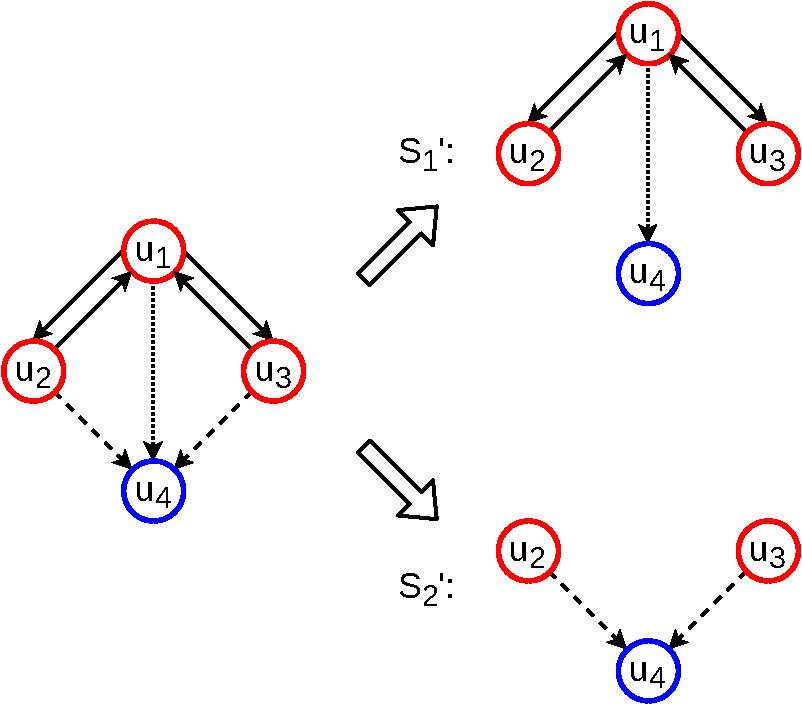
\includegraphics[width=0.35\textwidth]{img/stwig.pdf}
  \caption{Stars generated by existing algorithms.}\label{img:stwig}
\end{figure}
The edge $u_1 \rightarrow u_4$ is lost in $S_2'$.
Therefore, vertex $10$ will be matched (Figure~\ref{img:running_example}) which is unnecessary.
The problem is more severe for complex patterns where more edges need to be discarded.

SeqStar addresses the problem by keeping the original pattern graph unchanged, and removing vertices/edges on a copy $p'$ of the pattern (Algorithm~\ref{alg:decompose_stars}).
Algorithm~\ref{alg:decompose_stars} is similar to the vertex-cover selection algorithm~\cite{DBLP:books/daglib/0023376}.
The set $R$ in Algorithm~\ref{alg:decompose_stars} stores the candidate root vertices.
The algorithm uses a heuristic function $f(u) = \frac{\deg(u) + |\psi(u)|}{\operatorname{freq}(u.label)}$ to select roots,
where $\deg(u)$ is the degree of $u$, $|\psi(u)|$ is the number of constraints related to $u$ ($u_2 > u_1$, $u_3 > u_1$, $u_4 < 8$ in Figure~\ref{img:running_example}),
and $\operatorname{freq}(u.label)$ is the frequency of $u$'s label in the data graph.
By maximizing the function $f$,
SeqStar prefers vertex that
(1) has a high degree and has more associated constraints,
(2) has a less popular label in the data graph.
Therefore, the size of intermediate results from star matching can be reduced.
The neighbors of the selected root will then be added to the candidate set $R$.
By doing so, the roots selected by Algorithm~\ref{alg:decompose_stars} will be connected and forms a \emph{connected vertex-cover}.
And we'll use this property to build index for join operation~\ref{sec:match_join}.
Finally, SeqStar uses the selected root to extract stars from the original pattern graph $p$.
$\operatorname{Star}(p, root)$ is obtained by copying all the edges connected with $root$.
Therefore, all the structural information of $p$ is inherited to the stars.
%TODO:这里加讨论,这两条的点在之后的匹配中能够起到什么作用。

  %% Consider the pattern graph in Figure~\ref{img:star_decomposition},
  %% suppose that $u_1$, $u_2$ and $u_3$ are selected as the roots,
  %% existing decomposition method would result in three stars with 3, 2 and 1 neighbor\@(s)
  %% by consecutively selecting and removing vertices from the original pattern.
  %% However, many useful matching information are lost by doing so,
  %% e.g., the third ``star'' is just an edge, which would generate enormous unnecessary matching results whereas every edge in the data graph would match it but only a part of them could match the original pattern graph.
  %% In contrast, our approach (Algorithm~\ref{alg:decompose_stars}) would keep all the neighborhood matching information as is shown in the bottom of Figure~\ref{img:star_decomposition}, which could then reduce unnecessary intermediate results significantly (Section~\ref{sec:experiments}).
  %% Like previous work~\cite{DBLP:journals/pvldb/SunWWSL12}, we also use a heuristic function to select a join order, which is defined as $ f(u) = \frac{\deg(u) + |\psi(u)|}{\operatorname{freq}(u.label)} $, i.e.,
  %% we prefer to select vertex with bigger degree (more early filters) and less label frequency (smaller intermediate matching results) first.
  %% $|\psi(u)|$ is the number of local constraints of $u$, which will be discussed further in Section~\ref{sec:match_optimize}.
  %% The root candidate set $R$ is used to select a connected vertex cover,
  %% which could then be joined efficiently (Section~\ref{sec:match_join}).
  %% The key feature of the algorithm is to remove selected vertex in a copy $p'$ of the pattern and always keeps the original useful information in $p$, and thus, the intermediate results of our star could be much smaller.
  %% \begin{figure}[ht]
  %%   \centering
  %%   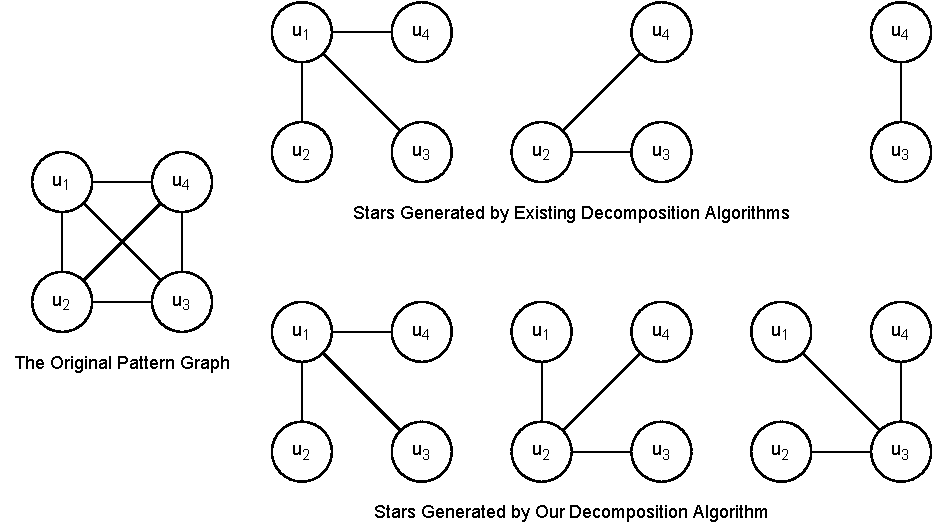
\includegraphics[width=0.48\textwidth]{img/star_decomposition.pdf}
  %%   \caption{Stars decomposed from the same pattern graph using different algorithms.}\label{img:star_decomposition}
  %% \end{figure}
%% \end{enumerate}
\begin{algorithm}[ht]
  \caption{Star Decomposition}\label{alg:decompose_stars}
  \SetKwFunction{DecomposeStars}{\textsc{DecomposeStars}}
  \SetKwFunction{Peek}{\textsc{Peek}}
  \SetKwFunction{Star}{\textsc{Star}}
  \SetKwFunction{RemoveVertex}{\textsc{RemoveVertex}}
  \Fn{\DecomposeStars{$p$}}{
    $stars \leftarrow \emptyset$\;
    $p' \leftarrow p$\;
    $R \leftarrow \{\max_{u \in V(p)}f(u)\}$\;
    \While{$R \neq \emptyset$}{
      $root \leftarrow \max_{u \in R}f(u)$\;
      $R \leftarrow R \setminus \{ root \}$\;
      $R \leftarrow R \cup \{ leaf \mid leaf \text{ is adjacent to } root \text{ in } p'\}$\;
      \RemoveVertex{$p'$, $root$}\;
      $R \leftarrow R \setminus \{ u \mid u \in p' \land \deg{u} = 0 \}$\;
      $stars \leftarrow stars \cup \{$ \Star{$p$, $root$} $\}$\;
    }
    \Return{$stars$}
  }
\end{algorithm}

To match a star $S$ on the vertex-centric storage engine,
SeqStar first seeks the \textsc{VertexIter} by searching the global index of the storage engine.
For each vertex $v$ in \textsc{VertexIter},
SeqStar first checks the degree of $v$ and applies constraints if available (\S\ref{sec:match_optimize}) to determine whether $v$ could be matched.
If $v$ passes these filters, SeqStar checks the neighbors of $v$ by visiting the \textsc{NeighborIter}.
For each neighbor vertex $n$ in \textsc{NeighborIter},
the in/out-edges associated with $n$ is compared to the corresponding leaf vertex of the star pattern.
The constraints extract from the WHERE clause will be applied to filter out unnecessary $n$ (\S\ref{sec:match_optimize}).
Since the iterators will only incur sequential data accesses,
the star matching process avoids the random disk seeks.

SeqStar adopts two techniques to further reduce the I/O cost:
(1) SeqStar analyzes the isomorphism among the stars to avoid redundant I/Os.
%% Some pattern may generate isomorphic stars, e.g., a triangle where each vertex has an edge point in and out.
Though the general graph isomorphism problem is NP complete, the isomorphism of stars are much easier to check.
We define an order for the vertices in a star based on the vertex labels. The isomorphism among stars can be checked by comparing the sorted stars.
Isomorphic stars have the same matching results. They only need to match once.
%and SeqStar will only match once for all.
(2) As the disk scanning operation is time consuming, it is preferable to scan it only once when solving a property graph matching problem.
SeqStar addresses the challenge by grouping stars with the same root label together,
and matches them in a single \textsc{VertexIter}.
For each scanned vertex $v$, SeqStar will check all the star patterns with the same root label as $v$.
Therefore, the graph data can be scanned only once without back and forth seeking.

%% Since the real-world graphs are so large that it is preferable to scan it only once when solving a property graph matching problem.
%% SeqStar solves the problem by grouping stars with the same root label together,
%% and scans these stars together by iterating through the \textsc{VertexIter}.
%% For each scanned vertex, SeqStar visits the \textsc{NeighborIter} to check the neighbors and stores the intermediate results for these stars.
%% Moreover, SeqStar is able to find isomorphism among stars and avoids unnecessary star matching (\S\ref{sec:match_optimize}).
%% However, it is not a simple task to match multiple stars in a single sequential scan,
%% the context switch cost and the intermediate result write cost must be minimized.
%% For the context switch cost, it is strongly coupled with the underlying storage method of the data graph.
%% Thanks to the elegant design of our vertex-centric storage model,
%% which is able to match stars in a sequential run given a root label,
%% we could group the stars with the same root label together and match them at the same time when iterating through \textsc{VertexIter}.
%% For the matching result write cost, we developed a compression algorithm for star's matching results that could be wrote sequentially (Section~\ref{sec:match_compress}).
%% As a result, we could scan the huge data graph only once and all the I/Os are sequential.

\subsection{Intermediate Results Compression}\label{sec:match_compress}
The matching results grow exponentially with respect to the size of the graph data.
%TODO:多次提到中间结果指数膨胀,最好在第一次出现的时候说点理由,从别人论文里面摘录出来也行
Consider the matching problem in Figure~\ref{img:running_example},
$S_1$ will generate 28 rows of intermediate results and $S_2$ will generate 8 rows.
And we need $4 \times (28 + 8) = 144$ integers to store them, which is larger than the data graph (10 vertices, 20 edges).
Inspired by the vertex-cover based compression algorithm~\cite{DBLP:journals/pvldb/QiaoZC17},
SeqStar postpones the costly Cartesian product and leveraging equivalence classes among vertices to reduce the size of intermediate results.
Moreover, we design an on-disk layout that is able to write the compressed data sequentially.

Two techniques are used to compress the intermediate results:
(1) Like VCBC, SeqStar avoids the Cartesian product in the intermediate results.
For each vertex $v$ that will match the root of a star $S$,
SeqStar stores the matched vertices of each neighbor of $v$ in $S$ together as an \emph{image set}.
They are then stored together as a \emph{SuperRow}.
For example, there are two SuperRows in $T_2$ (Figure~\ref{img:running_example}),
each contains a root vertex and two image sets.
(2) SeqStar analyzes the vertices in stars and use equivalence classes to avoid unnecessary storage.
SeqStar first groups the leaf vertices by label.
It then studies the connections between the leaves and the root.
Vertices have the same edge properties (direction, labels) and filtering function are grouped together as a \emph{neighbor equivalence class},
e.g., $u_2$ and $u_3$ in Figure~\ref{img:running_example}.
The matching results of the vertices are the same, and SeqStar stores their image set only once.
As a result, SeqStar uses only 16 integers to store the compressed intermediate results in Figure~\ref{img:running_example}.
\begin{figure}[ht]
  \centering
  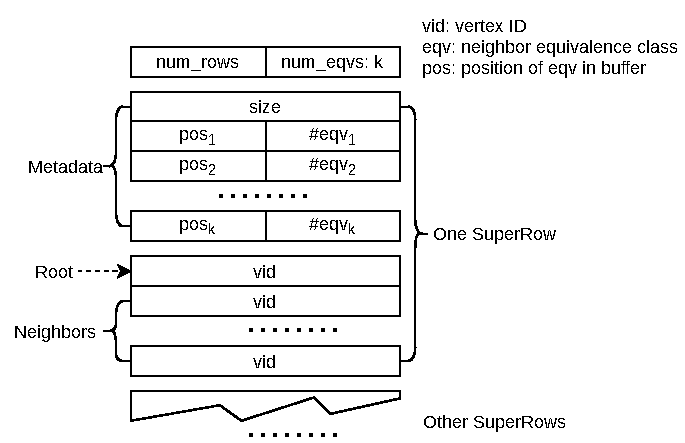
\includegraphics[width=0.45\textwidth]{img/compress.pdf}
  \caption{On-disk layout of the compressed intermediate results.}\label{img:compress}
\end{figure}

Figure~\ref{img:compress} shows the SuperRows' on-disk layout.
In each SuperRow, the matched vertices are stored consecutively.
Metadata $(pos_i, \#eqv_i)$, $ 1 \le i \le k$, are used to store the image sets for each neighbor equivalence class.

During the star matching process, matched vertices from the \textsc{NeighborIter} will be appended to the SuperRow file.

%% VCBC groups the matching results by the vertex-cover and stores the matched vertices in \emph{image sets}.
%% The original data can be restored by doing Cartesian product on the image sets.
%% As a result, only 16 integers are required
%% The compression ratio of the algorithm is as high as $10^{10}$ (\S\ref{sec:experiments_compress}).

% As our experiment shows that a small graph with $10^5$ edges could easily results in $10^{10}$ rows of matching results (Section~\ref{sec:experiments}).
%% Even though we could use stars and auxiliary optimizations to drop out useless matching results as soon as possible, the intermediate results could still be very large.
%% Figure~\ref{img:compress_example} illustrates this phenomenon that a small graph with only 6 vertices could result in 12 rows (48 vertices) of matching results.
%% In the table we could find that $u_1$ and $u_4$ always match the same vertices $v_2$ and $v_1$,
%% whereas the matching results of $u_2$ and $u_3$ are permutations of $v_3, v_4, v_5, v_6$.
%% \emph{The key of the matching result explosion problem is the explosive permutation}.
%% In order to address this problem, we avoid the permutation by postpone the Cartesian production when matching stars, which is similar to VCBC~\cite{DBLP:journals/pvldb/QiaoZC17} but we focus on the compression of property star's matching results for out-of-core systems.

%% Consider Figure~\ref{img:compress_example}, there is a symmetry with $u_2$ and $u_3$.
%% We say that they have the same \textsc{NeighborInfo} or they form a \textsc{NeighborInfo} equivalence class, as they have the same label and same connections to the root $u_4$,
%% and we can be sure that the matching results of $u_2$ and $u_3$ are always same.
%% The \textsc{NeighborInfo} of $u_1$ is different from $u_2$ because $u_1$ has more edges connected to the root.
%% By iterating through the neighbors of $v_1$, we can find the image set for each vertex in the pattern.
%% Instead of permuting the matching vertices, we compress the matching result by just writing down the image sets of each \textsc{NeighborInfo} equivalence class as is shown in the right bottom corner in Figure~\ref{img:compress_example}.
%% And Figure~\ref{img:compress} gives a straightforward disk format to store the compressed star matching results.
%% The final results can be retrieved by doing Cartesian product on the image sets and keeping the unique vertices.
%% We called the compressed data as \emph{SuperRow} since one SuperRow could generate enormous tuples by Cartesian production.
%% \begin{figure}[ht]
%%   \centering
%%   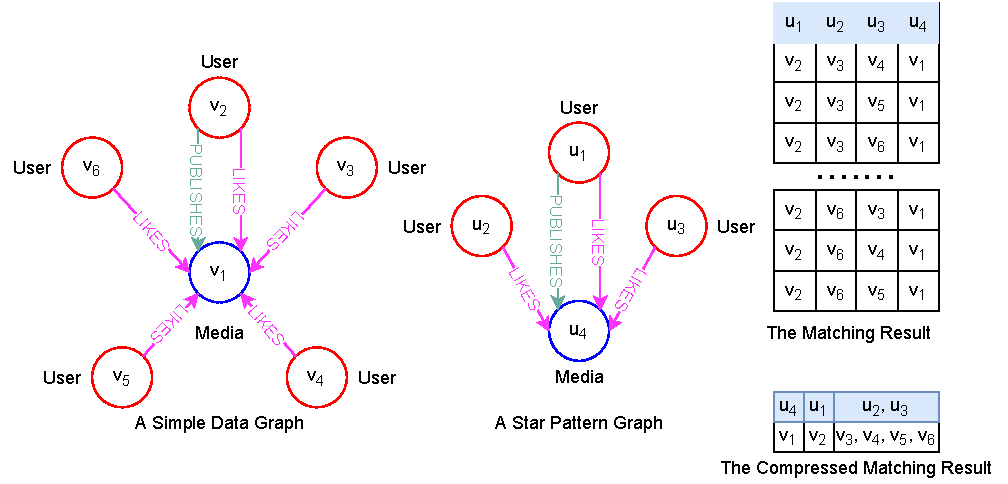
\includegraphics[width=0.53\textwidth]{img/compress_example.pdf}
%%   \caption{A small graph could results in enormous matching results.}\label{img:compress_example}
%% \end{figure}

%% However, there are still two challenges to be faced in practice:
%% 1. In real-world property graphs, as a celebrity vertex could have millions of neighbors, it could become a bottleneck if we have to scan the neighbors multiple times when matching a star;
%% 2. The SuperRows should be written sequentially to reduce the I/O cost.
%% If we want to scan the neighbors only once, we should be able to append the neighbor vertex to the corresponding image set, however, the variable-length image sets make it hard to address these problems.
%% To solve this dilemma, for each SuperRow, we pre-allocate enough space based on the statistical information in the data graph, i.e., the size of neighbors with the \textsc{NeighborInfo}'s label.
%% Thus the vertices could be scanned only once and wrote to the corresponding image set sequentially.

\subsection{Pipeline Join on Compressed Data}\label{sec:match_join}
%% By far, we've got all the compressed matching results for stars and it's time to join them to obtain the final answer.
%% A simple and straightforward method is the binary join, however, intermediate join results have to be materialized by doing so.
%% Even though the compression ratio of star matching result is very impressive,
%% the joined result could expand significantly because the permutation among roots is unavoidable~\cite{DBLP:journals/pvldb/SunWWSL12}.
%% To address this problem, we propose a indexed pipeline join algorithm on compressed data:
SeqStar reduces the memory usage further by performing pipeline join on compressed data.

To boost the join operation, we design an index on the SuperRow data.
Consider the SuperRow layout in Figure~\ref{img:compress}, each SuperRow contains only one root.
The uniqueness of the root makes it possible to be the key of a index (SuperRow-index):
Given a root ID, it returns the position of the corresponding SuperRow.
Since the vertices are sorted in the storage engine,
the SuperRow-index can be build by appending after a SuperRow is stored.
And the SuperRow-index operates by a simple binary search.

The planner of SeqStar first generate a join order based on the statistical parameters of SuperRows,
i.e., row number, average size of image sets.
The parameters are accumulated when a SuperRow is appended, and the cost is trivial.
Also note that in Algorithm~\ref{alg:decompose_stars}, the chosen root vertices form a connected vertex-cover.
The join order ensures the root of the stars are bound by previous stars.
For example, $T_1 \Join T_2 \Join \cdots \Join T_c$ (the discussion can be generalized to other join orders),
where $T_i$ is the SuperRows of $S_i$, and the root of $S_i$ is $u_i$.
SeqStar ensures $u_i \in V(S_{i-1})$ such that the Super-indexes will always work.

After that, SeqStar performs a pipeline join on the SuperRows to avoid materializing intermediate results.
The basic structure of the algorithm is a series of nested loops  (Algorithm~\ref{alg:join}).

\begin{algorithm}[ht]
  \caption{Pipeline Join}\label{alg:join}
  \SetKw{Yield}{yield}
  \ForEach{$sr_1 \in T_1$}{
    $v_1 \leftarrow sr_1[u_1]$\;
    \ForEach{$v_2 \in sr_1[u_2]$}{
      \If{$sr_2 \leftarrow T_2.idx(v_2)$}{
        \ForEach{$v_3 \in \bigcap_{u_3 \in sr}sr[u_3]$}{
          $\cdots$\;
          \If{$sr_c \leftarrow T_c.idx(v_c)$}{
            \Yield{$(v_1, \dots, v_c, \bigcap_{u_{c+1}\in sr}sr[u_{c+1}], \dots)$}\;
          }
        }
      }
    }
  }
\end{algorithm}

Unlike the traditional join problem, SeqStar joins on image sets rather than single elements.
That is to say set intersection is the most computation-intensive operation.
Since vertices are sorted in the storage engine,
the order will still preserves in every image sets.
This property makes it perfect for the merge algorithm to perform set intersection.
%% Consider the SuperRows in Figure~\ref{img:running_example}, whose columns are image set for \textsc{NeighborInfo} equivalence class except the first column, which is the matching result of the root.
%% Thus the first column of a SuperRow contains only a single vertex, which is suitable for the key of a index.
%% In fact, the index is generated during the star matching process,
%% for each SuperRow we append the root id and the position of it to the index file.
%% With this index, we are able to locate to the corresponding SuperRows efficiently during the join process.

%% The basic structure of our pipeline join is a series of nested loops.
%% However, unlike the traditional join problem, we join on image sets rather than single elements,
%% which means set intersection is the most computation intensive operation.
%% Consider the social media network, a trending media could easily attract millions or even billions of viewers,
%% to join on such trending media rooted stars, we must calculate the set intersection of such enormous viewers.
%% A conventional hash join method could easily eat up the memory of a PC and have poor locality.
%% To address this problem, we provide an out-of-core sequential approach by merging on the image sets.
%% Therefore the image sets should be sorted otherwise the sorting operation could be another bottleneck.
%% In fact, with the elegant design of our vertex-centric property graph storage method,
%% the vertices are already sorted in the data graph, and we can implement our sequential out-of-core set intersection for free.

\subsection{Optimizations}\label{sec:match_optimize}
In this section we discuss a series of optimizations for the property graph matching engine.
\subsubsection{Predicate Push Down}
The WHERE clause of a graph matching query specified a constraint or searching condition on the matching results.
The constraint are expressed in the form of predicates, e.g., $=$, $\neq$, $>$, $\ge$, $<$, $\le$.
And the Boolean operator AND ($\land$), OR ($\lor$), NOT ($\lnot$) can be used to combine multiple predicates into a new one.
For example, in Figure~\ref{img:cypher_query}, there are three predicates concatenated by AND\@.
Formally, the constraint is a function $\psi: PG \rightarrow B$ with $PG$ the set of pattern graph and $B$ the set of Boolean values.
We will also use $\psi$ to denote abstract predicate for simplicity in this section:
$\psi(u)$ defines a constraint $\psi$ on vertex $u$, e.g., ``{id(u4) >= 2020}'' defines a vertex constraint on $u_4$ where the ID of the matching vertex of $u_4$ must great than or equal to $2020$;
and $\psi(u_1, u_2)$ defines a constraint on vertex $u_1$ and vertex $u_2$,
e.g., ``{id(u1) < id(u2)}'' defines a constraint on $u_1$ and $u_2$ that the ID of the matching of $u_1$ must be less than that of $u_2$.

Previous work usually ignore the constraint specification part of a graph matching query.
If someone wants to query a pattern with a specific searching condition,
she or he has to match the pattern graph first and then filter on the matching results,
which leaves a lot of room for improvement because the user provided searching conditions could filter out many unnecessary
partial results in an early phase.

However, it is still challenging to make use of the constraint provided by user's WHERE clause.
The pattern graph and the constraint are logically two different things,
we have to obtain enough information in order to use the constraint as early filter during the graph matching phase.
For example, the constraint in Figure~\ref{img:cypher_query} include all the vertices in the pattern graph,
only when the pattern graph is already matched could we got enough information to apply the constraint,
which makes the constraint filter nearly useless.

\begin{figure}[ht]
  \centering
  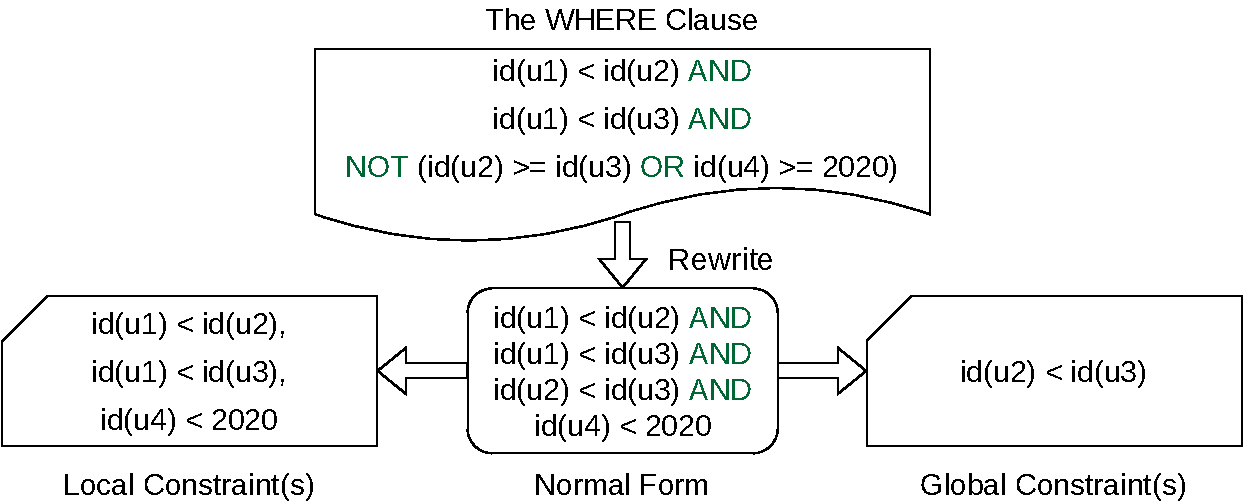
\includegraphics[width=.45\textwidth]{img/constraints.pdf}
  \caption{Constraint Analysis.}\label{img:constraints}
\end{figure}

To address this problem, as shown in Figure~\ref{img:constraints},
we dive into the syntax tree of the graph matching query and decompose the searching condition into smaller parts which require only what we could got during the graph matching phase.
Specifically, we decompose the searching condition into three parts: \emph{vertex constraints}, \emph{edge constraints} and \emph{global constraint}.
A vertex constraint is a function $\psi(u)$ mapping vertex $u$ to Boolean values,
and an edge constraint sets a constraint on edge $(u_1, u_2)$ by a function $\psi(u_1, u_2)$.
For example, in Figure~\ref{img:pattern_graph} ``{id(u4) < 2020}'' sets a vertex constraint on $u_4$,
``{id(u1) < id(u2)}'' and ``{id(u1) < id(u3)}'' are edge constraints,
while ``{id(u2) < id(u3)}'' is not because there is no edge between $u_2$ and $u_3$.
The \emph{vertex constraints} and \emph{edge constraints} are \emph{local constraints} that only require local information that can be obtained during the graph matching phase.
So they could then be pushed down to the data graph scanning phase to short-circuit useless matching results.
A global constraint $\psi(u_1, u_2, \dots)$ sets a constraint on a series of vertices $u_1, u_2, \dots$,
the information is insufficient during the data graph scanning phase.

\begin{algorithm}[ht]
  \caption{Constraint Rewriting}\label{alg:rewrite}
  \SetKwFunction{ConstraintRewrite}{\textsc{ConstraintRewrite}}
  \SetKwFunction{Simplify}{\textsc{Simplify}}
  \Input{$expr$: the abstract syntax tree of the WHERE clause}
  \Output{A set of simplified constraints connected by the AND ($\land$) operator}
  \Fn{\ConstraintRewrite{$expr$}}{
    \Match{$expr$}{
      \Case{$\lnot \lnot e$}{\Return{\ConstraintRewrite{$e$}}}
      \Case{$\lnot (e_1 \lor e_2)$}{
        \Return{\ConstraintRewrite{$\lnot e_1$} $\cup$ \ConstraintRewrite{$\lnot e_2$}}
      }
      \Case{$e_1 \land e_2$}{\Return{\ConstraintRewrite{$e_1$} $\cup$ \ConstraintRewrite{$e_2$}}}
      \Case{$e$}{\Return{$\{$ \Simplify{$e$} $\}$}}
    }
  }
\end{algorithm}

Logically, the AND ($\land$) operator create a new constraint $\psi = \psi_1 \land \psi_2$ by combining two constraints $\psi_1$ and $\psi_2$,
where $\psi_1$ and $\psi_2$ can be used to check the matching results independently because there is no side effects in constraints,
so we could safely split $\psi$ into $\psi_1$ and $\psi_2$.
Because local constraints are the earliest constraint filters, we should extract as much as possible.
In order to make the constraint filters more efficient and extract more local constraints:
Firstly, we optimize the AST by classic methods such as compile-time calculation,
handle special cases such as ``{WHERE false}''.
Then, we apply Algorithm~\ref{alg:rewrite} to analyze the syntax tree and rewrite it into \emph{normal form},
where a normal form is a list of simplified constraints connected by the AND operator.
In fact, the constraints are mostly specified by binary operators such as ``$\le$'', ``$\ne$'',
hence many constraints are naturally local constraints.
And the De Morgan's law enables us to convert the OR ($\lor$) operator into AND ($\land$):
\begin{equation}
  \lnot (\psi_1 \lor \psi_2) = \lnot \psi_1 \land \lnot \psi_2
\end{equation}
So Algorithm~\ref{alg:rewrite} will always keep the semantics of the original user provided constraint.
For example, the third predicate of the AND operator in Figure~\ref{img:cypher_query} would be rewritten to
\begin{verbatim}
  id(u2) < id(u3) AND id(u4) < 2020
\end{verbatim}
by applying De Morgan's law.
And the WHERE clause of Figure~\ref{img:cypher_query} would be rewritten to the normal form:
\begin{verbatim}
  WHERE id(u1) < id(u2) AND id(u1) < id(u3)
  AND id(u2) < id(u3) AND id(u4) < 2020
\end{verbatim}

\begin{algorithm}[ht]
  \caption{Constraint Pushdown}\label{alg:push_down}
  \SetKwFunction{ConstraintPushdown}{\textsc{ConstraintPushdown}}
  \SetKwFunction{AddVertexConstraint}{\textsc{AddVertexConstraint}}
  \SetKwFunction{AddEdgeConstraint}{\textsc{AddEdgeConstraint}}
  \SetKwFunction{Edges}{\textsc{Edges}}
  \Input{The normal form of constraints $exprs$ and the user described pattern graph $p$}
  \Output{The vertex constraints and edge constraints are pushed down to $p$ and the global constraints will be returned}
  \Fn{\ConstraintPushdown{$exprs$, $p$}}{
    $globals \leftarrow [\,]$\;
    \ForEach{$expr \in exprs$}{
      \Match{$expr$}{
        \Case{$\psi(u)$}{\AddVertexConstraint{$p$, $\psi(u)$}}
        \Case{$\psi(u_1, u_2)$}{
          \If{$(u_1, u_2) \in$ \Edges{$p$}}{\AddEdgeConstraint{$p$, $u_1$, $u_2$, $\psi(u_1, u_2)$}}
        }
        \Case{$e$}{$globals \leftarrow globals \cup \{e\}$\;}
      }
    }
    \Return{$globals$}
  }
\end{algorithm}

The normal form is then used to extract useful information to be pushed down to the pattern graph as in Algorithm~\ref{alg:push_down}.
For each constraint in the normal form, we check if it is local constraint and then push it down to the corresponding vertex or edge.
After that, We could then decompose it into stars.
Our framework contains a JIT compiler that is able to emit callable closures based on the AST,
and the local constraints can then be used to serve as early filters in the data graph scanning process to short-circuit unnecessary matchings as soon as possible.
\subsubsection{Star Isomorphism}
Consider Figure~\ref{img:star_decomposition}, we generate three stars from the original pattern,
and these stars are isomorphic with each other.
Therefore the matching results of these stars are always the same,
there is no need to match these stars again and again.
Though the general graph isomorphism problem is NP complete,
the isomorphism of stars are easier to check.
We say that our stars in Figure~\ref{img:star_decomposition} belong to the same \textsc{Characteristic} equivalence class,
where \text{Characteristic} is a structure that stores the root and neighbors in a predefined order.
By grouping isomorphic stars into the same \textsc{Characteristic} equivalence class,
we could avoid unnecessary computation.


\section{Evaluation}\label{sec:experiments}
\subsection{Setup}
\subsubsection{Environment}
The experiments were performed on a single machine with two Intel Xeon Processor E5--2699 v4 CPUs, 64 GB of RAM,
and a 800GB SSD\@.
The machine has 22 cores and 44 threads.
Memory caches were dropped before each experiment to force disk loads.
\subsubsection{Datasets and Queries}
We use real-world data graphs~\cite{snapnets} listed in Table~\ref{tab:datasets}.
The datasets come from difference domains of application, and they range in different size.
The vertices and edges in the datasets are labeled randomly as in~\cite{DBLP:journals/pvldb/MhedhbiS19}.

The queries (Figure~\ref{img:queries}) are selected and edited from existing work~\cite{DBLP:conf/cloud/SerafiniMS17,DBLP:journals/pvldb/MhedhbiS19}.
The labels of vertices and edges are tagged randomly,
and they are represented by the color and the style of lines in Figure~\ref{img:queries}.
The queries we choose represent different topologies: trees, chains, and cyclic graphs.
$q_9$ --- $q_{12}$ are queries with multi-edges.
\begin{table}
  \caption{Datasets}\label{tab:datasets}
  \begin{tabular}{lrr}
    \toprule
    Name & $|V|$ & $|E|$ \\
    \midrule
    soc-Epinions (EP) & 76K & 509K \\
    web-Google (GO) & 876K & 5.1M \\
    web-BerkStan (BS) & 685K & 7.6M \\
    soc-LiveJournal (LJ) & 4.8M & 69M \\
    com-Orkut (OK) & 3.1M & 117.2M \\
    \bottomrule
  \end{tabular}
\end{table}

\begin{figure}[ht]
  \centering
  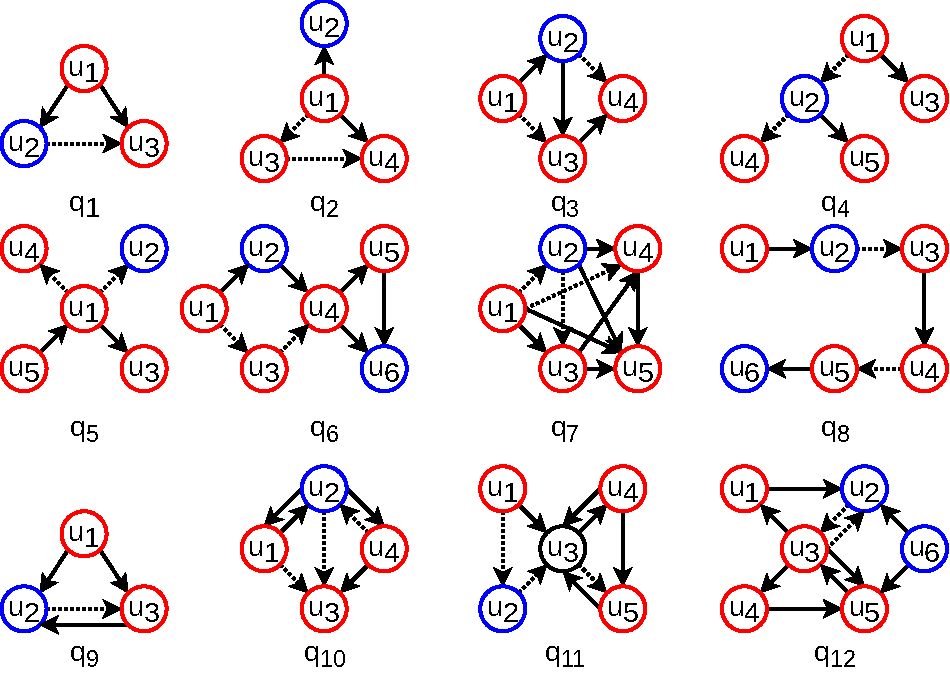
\includegraphics[width=0.5\textwidth]{img/queries.pdf}
  \caption{The queries.}\label{img:queries}
\end{figure}

\subsection{Preprocessing Cost}
We first study the preprocessing cost of SeqStar's vertex-centric storage engine.
The preprocessing incurs a external sort on the original graph data to generate the formatted data graph shown in Figure~\ref{img:data_graph}.
The cost is $\mathcal{O}(n \log n)$ where n is the size of the unsorted graph data.
We use 32-bit integers to store the vertex IDs, and 16-bit integers to store the vertex/edge labels.
As is shown in Figure~\ref{img:exp_preprocessing}, the preprocessing time grows linearly with respect to the size of graph data.
In fact, the preprocessing time of the vertex-centric storage is significantly smaller than the execution time of complex queries.

\begin{figure}[ht]
  \centering
  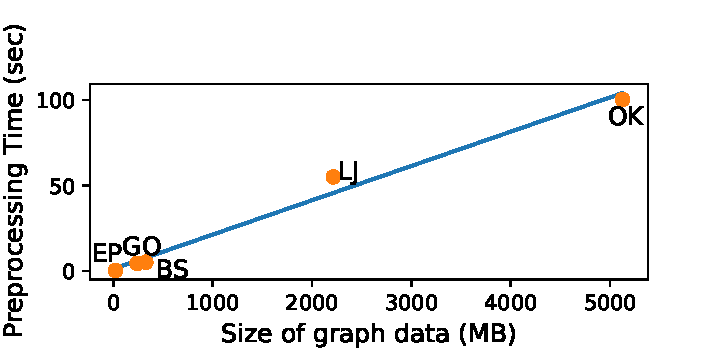
\includegraphics[width=0.4\textwidth]{img/exp_preprocessing.pdf}
  \caption{Preprocessing time of SeqStar.}\label{img:exp_preprocessing}
\end{figure}
\subsection{Comparative Performance}
We compare the overall performance of SeqStar against Graphflow~\cite{DBLP:journals/pvldb/MhedhbiS19} and Neo4j.

Graphflow is the state-of-the-art in-memory subgraph querying system,
and it is the fastest baseline we are aware of.
Graphflow is a JVM based system, and we set the maximum size of the JVM heap to 60GB to let it make full use of main memory.
However Graphflow does not support queries with multi-edges, i.e., $q_9$ --- $q_{12}$,
and it will report fake results for these queries\footnote{Graphflow will report matchings even the data does not contain multi-edges.}.
Therefore we use only $q_1$ --- $q_8$ to compare with Graphflow.
\begin{figure*}[ht]
  \centering
  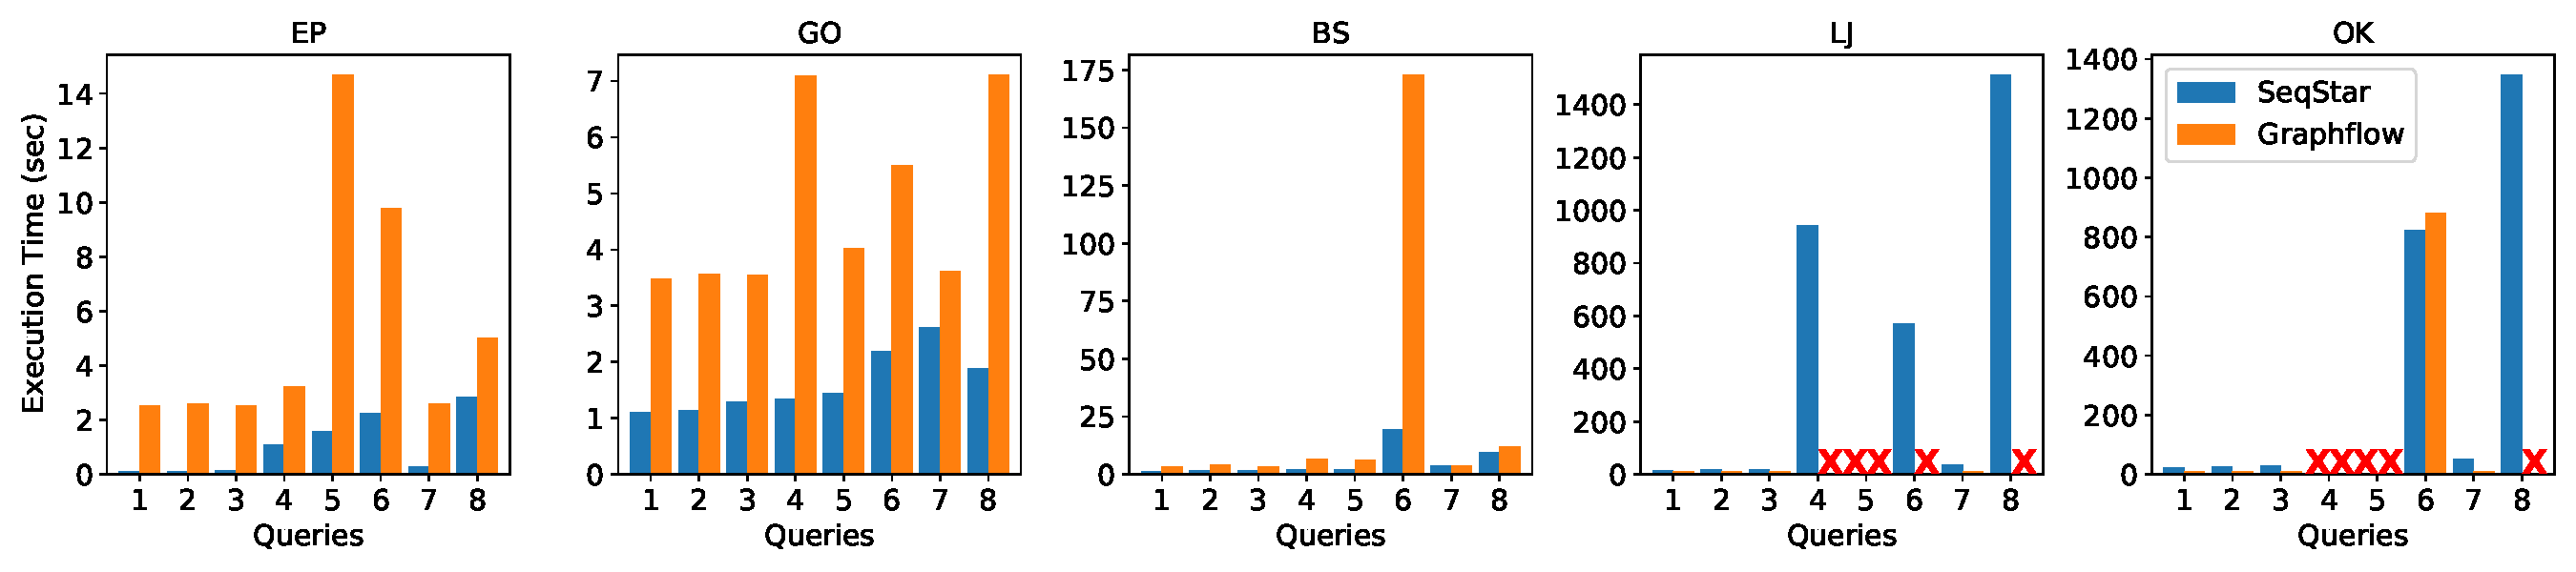
\includegraphics[width=\textwidth]{img/exp_compare.pdf}
  \caption{Execution time.}\label{img:exp_compare}
\end{figure*}

\subsection{Compression Ratio}
\subsection{Performance of Star Decompression}
\subsection{Parallelism of Pipeline Join}

\section{Related Work}
Despite the fact that general property graph matching problem is seldom discussed in previous works,
simple graph matching has been widely studied.
We survey these relevant work in this section.
\subsection*{In-memory Methods}
Most of the early work assumes that the data graph and indices are fit in the main memory of a single machine.
Sparked by Ullmann's backtracking algorithm~\cite{DBLP:journals/jacm/Ullmann76},
many subgraph matching algorithms have been proposed using different searching order, filter rules, and neighborhood indices~\cite{DBLP:journals/pami/CordellaFSV04,DBLP:journals/pvldb/ShangZLY08,DBLP:conf/sigmod/HeS08,DBLP:conf/sigmod/HanLL13,DBLP:journals/pvldb/LeeHKL12}.
These algorithms usually use a DFS-style tree-based graph exploration to search the matchings without materializing intermediate results.
However, these single machine in-memory algorithms are no longer suitable for nowadays billion-node graphs.

To address the scalability problem of single machine in-memory algorithms,
many distributed subgraph matching algorithms have been proposed~\cite{DBLP:journals/pvldb/SunWWSL12,DBLP:conf/sigmod/ShaoCCMYX14,DBLP:journals/pvldb/LaiQLC15,DBLP:journals/pvldb/LaiQLZC16,DBLP:conf/cloud/SerafiniMS17}.
Because the vertices of the data graph are scattered among machines,
these algorithms usually match smaller patterns and get the final result by join operation.
For example, Sun et al.~\cite{DBLP:journals/pvldb/SunWWSL12} introduce a star-like basic matching unit called STwig,
and implement their subgraph matching algorithm on top of the Trinity~\cite{shao2012the} memory cloud.
Lai et al.~\cite{DBLP:journals/pvldb/LaiQLC15} propose TwinTwig join using MapReduce,
where a TwinTwig is either a single edge or two incident edges of a vertex.
The SEED~\cite{DBLP:journals/pvldb/LaiQLZC16} algorithm use both star and clique as the join units,
and use clique compression technique to further improve the performance.
However, these distributed algorithms still suffer from severe memory crisis,
because the size of partial results grow exponentially with respect to the size of the date graph.
Moreover, they must be transferred to other machines before join,
which is the most expensive operation in a parallel system such as MapReduce.

Besides, the optimization of a subgraph matching algorithm relies heavily on the underlying graph model:

Unlabeled undirected simple graph is perhaps the simplest graph model,
which can be viewed as a special case of property graph with all the vertices and edges have the same label and have no multi-edges.
Some authors distinguish this kind of graphs from others and designate the matching problem of this kind of graph as \emph{subgraph listing}~\cite{DBLP:conf/sigmod/ShaoCCMYX14,DBLP:journals/jacm/Ullmann76,DBLP:conf/sigmod/ShaoCCMYX14,DBLP:journals/pvldb/LaiQLC15,DBLP:conf/sigmod/KimLBHLKJ16,DBLP:journals/pvldb/LaiQLZC16,DBLP:journals/pvldb/QiaoZC17}.
CBF~\cite{DBLP:journals/pvldb/QiaoZC17} is the state-of-the-art subgraph listing algorithm,
which decompose the pattern graph into a several basic structures called \emph{crystals},
and match these basic units with partial results compressed by the VCBC algorithm.
However, it is unable to support general property graph because CBF relies on clique listing to match crystals,
which implies the equivalence of vertices in a clique (complete graph) and is not the case of property graph model because of labels and direction of edges.

Another widely studied graph model is vertex-labeled undirected simple graph~\cite{DBLP:journals/pvldb/ShangZLY08,DBLP:journals/pvldb/SunWWSL12,DBLP:conf/sigmod/HanLL13,DBLP:conf/cloud/SerafiniMS17,DBLP:conf/sigmod/DiasTGM019}.
Turbo\textsubscript{ISO}~\cite{DBLP:conf/sigmod/HanLL13}, for example, is turbocharged by the concept of \emph{neighborhood equivalence class} (NEC).
It outperforms other competitors by safely avoid the permutation of all possible vertices in the same NEC\@.
A NEC is a set of vertices in the pattern graph, where every vertex has the same label and the same set of neighbors.
However, things become more complex and make it not suitable for the property graph model.
Because one has to check the labels of vertices, labels of edges, directions of edges in order to test the isomorphism of a property graph, and the real-world multigraphs make life even harder.
\subsection*{Out-of-core Methods}
Many out-of-core triangle enumeration algorithms have been proposed~\cite{DBLP:conf/kdd/ChuC11,DBLP:conf/osdi/KyrolaBG12,DBLP:conf/sigmod/HuTC13,DBLP:conf/sigmod/KimHLPY14}.
However, all these algorithms only deal with triangulation, a special case of the graph matching problem.
Recently, \textsc{DualSim}~\cite{DBLP:conf/sigmod/KimLBHLKJ16} take a further step and is able to match general unlabeled undirected graphs.
To avoid the materialization of intermediate results,
it fixes the data vertices by fixing a set of disk pages and then find all matchings in these pages.
Apparently, every page of the data graph must be swapped in/out many times in order to get the final result,
which lead to severe I/O cost.
In contrast, our approach will load the pages sequentially at most once,
and we can also use the compressed partial results to boost afterward queries.

\section{Conclusion}\label{sec:conclusion}
\textcolor{red}{This paper proposes SeqStar, an out-of-core property graph matching system.}
%This paper proposes SeqStar, which is the first out-of-core property graph matching system.
SeqStar uses the vertex-centric storage engine to store the information related to one vertex together.
This storage engine avoids the random disk access problemand provides the convenient iterators for programs to visit the required vertices.
Small indexes are designed to further minimize the number of IO operations.
For the graph matching engine,
SeqStar uses a novel star decomposition algorithm that preserves as much filtering information as possible in decomposed stars from the pattern graph.
Predicate pushdown is applied to further reduce unnecessary matchings.
In order to reduce the memory usage, SeqStar compresses the intermediate results by postponing Cartesian product and combining equivalent vertices.
And SeqStar performs parallel pipeline join on the compressed data to avoid unnecessary intermediate results.
Experimental results demonstrate that SeqStar outperforms existing work and is able to run more complex property graph queries with less memory consumption.


Currently, SeqStar lacks the support for dynamic graphs.
This limitation gives us directions for future work,
and we are now working on implementing the dynamic vertex-centric storage model to support dynamic graphs.
% 这里扯了一下 future work,看其他的 VLDB 都要在这说,甚至有的这整章就是 future work


%\clearpage
\balance{}
\bibliographystyle{ACM-Reference-Format}
\bibliography{refs}

\end{document}
\endinput
